%===============================================================================
% LaTeX sjabloon voor de bachelorproef toegepaste informatica aan HOGENT
% Meer info op https://github.com/HoGentTIN/latex-hogent-report
%===============================================================================

\documentclass[dutch,dit,thesis]{hogentreport}

% TODO:
% - If necessary, replace the option `dit`' with your own department!
%   Valid entries are dbo, dbt, dgz, dit, dlo, dog, dsa, soa
% - If you write your thesis in English (remark: only possible after getting
%   explicit approval!), remove the option "dutch," or replace with "english".

\usepackage{lipsum} % For blind text, can be removed after adding actual content

%% Pictures to include in the text can be put in the graphics/ folder
\graphicspath{{../graphics/}}

%% For source code highlighting, requires pygments to be installed
%% Compile with the -shell-escape flag!
%% \usepackage[chapter]{minted}
%% If you compile with the make_thesis.{bat,sh} script, use the following
%% import instead:
\usepackage{listings}
\lstset{
    basicstyle=\ttfamily\small, % Use monospaced font
    keywordstyle=\color{blue}\bfseries, % Keywords in bold blue
    commentstyle=\color{gray}, % Comments in gray
    stringstyle=\color{red}, % Strings in red
    numbers=left, % Line numbers on the left
    numberstyle=\tiny\color{gray}, % Line number style
    stepnumber=1, % Line number step
    breaklines=true, % Automatic line breaking
    frame=single, % Frame around the code
    captionpos=b, % Caption position (bottom)
    tabsize=4, % Tab size
    showstringspaces=false % Don't show spaces in strings
}
\usepackage[chapter,outputdir=../output]{minted}
\usemintedstyle{solarized-light}

%% Formatting for minted environments.
\setminted{%
    autogobble,
    frame=lines,
    breaklines,
    linenos,
    tabsize=4
}

%% Ensure the list of listings is in the table of contents
\renewcommand\listoflistingscaption{%
    \IfLanguageName{dutch}{Lijst van codefragmenten}{List of listings}
}
\renewcommand\listingscaption{%
    \IfLanguageName{dutch}{Codefragment}{Listing}
}
\renewcommand*\listoflistings{%
    \cleardoublepage\phantomsection\addcontentsline{toc}{chapter}{\listoflistingscaption}%
    \listof{listing}{\listoflistingscaption}%
}

% Other packages not already included can be imported here

%%---------- Document metadata -------------------------------------------------
% TODO: Replace this with your own information
\author{Thibo Haezaert}
\supervisor{Dhr. G. Blondeel}
\cosupervisor{Dhr. D. Mussen}
\title[]%
    {Hoe kan trust management effectief worden geïmplementeerd voor het beveiligen van bedrijven met heterogene gesegmenteerde netwerken?}
\academicyear{\advance\year by -1 \the\year--\advance\year by 1 \the\year}
\examperiod{1}
\degreesought{\IfLanguageName{dutch}{Professionele bachelor in de toegepaste informatica}{Bachelor of applied computer science}}
\partialthesis{false} %% To display 'in partial fulfilment'
%\institution{Internshipcompany BVBA.}

%% Add global exceptions to the hyphenation here
\hyphenation{back-slash}

%% The bibliography (style and settings are  found in hogentthesis.cls)
\addbibresource{bachproef.bib}            %% Bibliography file
\addbibresource{../voorstel/voorstel.bib} %% Bibliography research proposal
\defbibheading{bibempty}{}

%% Prevent empty pages for right-handed chapter starts in twoside mode
\renewcommand{\cleardoublepage}{\clearpage}

\renewcommand{\arraystretch}{1.2}

%% Content starts here.
\begin{document}

%---------- Front matter -------------------------------------------------------

\frontmatter

\hypersetup{pageanchor=false} %% Disable page numbering references
%% Render a Dutch outer title page if the main language is English
\IfLanguageName{english}{%
    %% If necessary, information can be changed here
    \degreesought{Professionele Bachelor toegepaste informatica}%
    \begin{otherlanguage}{dutch}%
       \maketitle%
    \end{otherlanguage}%
}{}

%% Generates title page content
\maketitle
\hypersetup{pageanchor=true}

%%=============================================================================
%% Voorwoord
%%=============================================================================

\chapter*{\IfLanguageName{dutch}{Woord vooraf}{Preface}}%
\label{ch:voorwoord}

%% TODO:
%% Het voorwoord is het enige deel van de bachelorproef waar je vanuit je
%% eigen standpunt (``ik-vorm'') mag schrijven. Je kan hier bv. motiveren
%% waarom jij het onderwerp wil bespreken.
%% Vergeet ook niet te bedanken wie je geholpen/gesteund/... heeft

In de voorbije 3 jaren van mijn studies in toegepaste informatica heb ik veel mogen bijleren, dankzij deze kennis mocht mijn passie voor IT nog meer groeien. 
In mijn laatste jaar kreeg ik de kans om bij KBC mijn stage te lopen, waar ik al gauw zag dat naast mijn opleiding nog veel kon worden bijgeleerd. \\

Binnen deze stage leerde ik veeltal bij over certificate authorities en public key infrastructures, technologieën die een cruciale rol hebben in de werking van digitale communicatie, maar waarvan ik alleen beschikte over de basiskennis.
Mijn co-promotor, Dirk Mussen, wie ook mijn stagementor was, bracht mij dan ook het idee voor het onderzoeksonderwerp van deze bachelorproef. Een onderwerp dat een actueel probleem aanhaalt die vele bedrijven en organisaties treft.
Dankzij de kennis opgedaan tijden mijn opleiding, stage en de begeleiding van mijn co-promotor, was het begrijpen en aanpakken van dit probleem een stuk eenvoudiger. \\

Bij deze wil ik mijn co-promotor graag bedanken voor zijn begeleiding en steun tijdens het uitvoeren van dit onderzoek. 
Naast mij co-promotor bedank ik ook graag mijn promotor, Gilles Blondeel voor het geven van feedback op deze paper alsook tips voor het mogelijks presenteren van deze bachelorproef.
Ik bedankt ook graag alle andere docenten die ik doorheen mijn opleiding heb mogen ontmoeten, voor de kennis die zij met mij hebben gedeeld.
%%=============================================================================
%% Samenvatting
%%=============================================================================

% TODO: De "abstract" of samenvatting is een kernachtige (~ 1 blz. voor een
% thesis) synthese van het document.
%
% Een goede abstract biedt een kernachtig antwoord op volgende vragen:
%
% 1. Waarover gaat de bachelorproef?
% 2. Waarom heb je er over geschreven?
% 3. Hoe heb je het onderzoek uitgevoerd?
% 4. Wat waren de resultaten? Wat blijkt uit je onderzoek?
% 5. Wat betekenen je resultaten? Wat is de relevantie voor het werkveld?
%
% Daarom bestaat een abstract uit volgende componenten:
%
% - inleiding + kaderen thema
% - probleemstelling
% - (centrale) onderzoeksvraag
% - onderzoeksdoelstelling
% - methodologie
% - resultaten (beperk tot de belangrijkste, relevant voor de onderzoeksvraag)
% - conclusies, aanbevelingen, beperkingen
%
% LET OP! Een samenvatting is GEEN voorwoord!

%%---------- Nederlandse samenvatting -----------------------------------------
%
% TODO: Als je je bachelorproef in het Engels schrijft, moet je eerst een
% Nederlandse samenvatting invoegen. Haal daarvoor onderstaande code uit
% commentaar.
% Wie zijn bachelorproef in het Nederlands schrijft, kan dit negeren, de inhoud
% wordt niet in het document ingevoegd.

\IfLanguageName{english}{%
\selectlanguage{dutch}
\chapter*{Samenvatting}

\selectlanguage{english}
}{}

%%---------- Samenvatting -----------------------------------------------------
% De samenvatting in de hoofdtaal van het document

\chapter*{\IfLanguageName{dutch}{Samenvatting}{Abstract}}


Het beheren van alle truststores en hun trust (de root certificaten die men vertrouwt), binnen een netwerk kan een tijdrovende taak zijn voor bedrijven. Zeker als het gaat over verschillende end-points met verschillende besturingssystemen, waarbij niet elke end-point dezelfde root certificaten nodig heeft.
Het is belangrijk dat bedrijven de root certificaten die ze gebruiken goed beheren, omdat deze certificaten bepalen welke communicatiesystemen vertrouwd worden en welke niet. 
Het vertrouwen van onnodige certificaten kan leiden tot een verhoogd risico op cyberaanvallen, terwijl het niet vertrouwen van noodzakelijke certificaten kan leiden tot een operationeel risico door het niet kunnen bereiken van bepaalde bronnen. \\

De vraag die deze bachelorproef beantwoorde is hoe bedrijven de truststores van hun systemen kunnen beheren, waarbij er rekening gehouden wordt met de verschillende besturingssystemen en de verschillende netwerksegmenten binnen een netwerk.
Deze bachelorproef streeft ernaar om deze vraag te beantwoorden door het leveren van een oplossingen die bedrijven kunnen gebruiken voor het beheren van de systeem truststores van Windows en Linux end-points.
Daarnaast worden er ook aanbevelingen gegeven voor bedrijven die deze oplossingen willen implementeren in hun infrastructuur. \\

Om tot deze oplossing te komen, werd er eerst een literatuurstudie uitgevoerd die belangrijke concepten en achtergrond informatie aanhaalde en daarnaast ook veel voorbereidende informatie gaf voor het ontwerpen van een oplossing.
Na een literatuurstudie werd een proof-of-concept opgezet waarin verschillende tools voor trust management werden getest.
%Deze omgeving is heterogeen, wat betekend dat er zowel Windows als Linux end-points aanwezig zijn. Ook is er segmentatie toegepast, met als doel dat systemen binnen hetzelfde netwerksegment dezelfde root certificaten vertrouwen. \\

In de proof-of-concept omgeving werden er voor beide Linux als Windows end-points 2 mogelijke oplossingen gevonden.
Bij Windows werd er gebruik gemaakt van Group Policy Objects (GPO's) voor de eerste oplossing en System Center Configuration Manager (SCCM) voor de tweede oplossing.
%Alhoewel de GPO's een gebruiksvriendelijke oplossing zijn, is het niet mogelijk om het toevoegen of verwijderen van root certificaten in de GPO's te automatiseren met Powershell, wat ervoor zorgt dat dit manueel moet gebeuren. Dit is niet schaalbaar bij een groot aantal root certificaten. Ook worden de GPO's enkel toegepast bij opstart of uitvoeren van een commando, wat ervoor zorgt dat de root certificaten niet altijd up-to-date zijn.
%SCCM biedt de mogelijkheid aan om Powershell scripts op regelmatige basis uit te voeren op de Windows end-points, wat ervoor zorgt dat de root certificaten vaker up-to-date zijn. Daarnaast kan er een Hashicorp Vault gebruikt worden om de root certificaten op een centraal punt op te slaan en beheren, zo kan het Powershell script de root certificaten uit de Vault halen en deze toevoegen aan de truststore van de Windows end-points. \\
Bij Linux werd in de eerste oplossing gewerkt met Ansible en later bij de tweede oplossing met Chef. 
%Ansible kan aan de hand van een oplijsting van end-points en instructies om root certificaten over te kopieren naar de truststores de truststores beheren via SSH verbindingen. Ansible legt alle verantwoordelijkheid bij de Ansible node zelf, wat ervoor kan zorgen dat bij een groot aantal end-points het een lange tijd kan duren tot de root certificaten vernieuwd zijn.
%Chef daarentegen laat de end-points zelf de instructies uitvoeren, wat het mogelijk maakt een groter aantal end-points op een snellere manier te beheren. De chef cookbooks kunnen dan ook gebruikt maken van de Hashicorp Vault om de root certificaten van de halen. \\
Beide oplossingen hebben hun eigen voor- en nadelen, maar hun toepasbaarheid hangt af van de infrastructuur van een bedrijf en hun voorkeuren. \\

De oplossing kan eenvoudig aangepast worden, zodat het bepalen van vertrouwde root certificaten niet beperkt blijft tot netwerksegmentatie, maar ook op basis van andere criteria kan gebeuren.
Daarnaast werden er nog een aantal aanbevelingen gegeven zoals het afstemmen van de truststore updates met activiteiten van een bedrijf hun bestaande PKI's en het verder onderzoeken van de mogelijkheden van de oplossingen op een grotere schaal. \\

%De scope en tijdsbeperking van deze bachelorproef hebben ervoor gezorgd dat er niet gekeken werd naar de security van de oplossingen, maar dat deze wel een basis kunnen leggen voor bedrijven om verder onderzoek te doen naar de security van hun truststores.
%Dit onderzoek heeft ook geen oog gehad voor IoT devices hun truststores of MacOS systemen, deze zouden dus ook nog verder onderzocht moeten worden door de bedrijven zelf.

Door de beperkte scope werd niet ingegaan op security-aspecten, IoT-devices of MacOS-systemen. Deze onderwerpen bieden kansen voor verder onderzoek.


%---------- Inhoud, lijst figuren, ... -----------------------------------------

\tableofcontents

% In a list of figures, the complete caption will be included. To prevent this,
% ALWAYS add a short description in the caption!
%
%  \caption[short description]{elaborate description}
%
% If you do, only the short description will be used in the list of figures

\listoffigures

% If you included tables and/or source code listings, uncomment the appropriate
% lines.
\listoftables

\listoflistings

% Als je een lijst van afkortingen of termen wil toevoegen, dan hoort die
% hier thuis. Gebruik bijvoorbeeld de ``glossaries'' package.
% https://www.overleaf.com/learn/latex/Glossaries

%---------- Kern ---------------------------------------------------------------

\mainmatter{}

% De eerste hoofdstukken van een bachelorproef zijn meestal een inleiding op
% het onderwerp, literatuurstudie en verantwoording methodologie.
% Aarzel niet om een meer beschrijvende titel aan deze hoofdstukken te geven of
% om bijvoorbeeld de inleiding en/of stand van zaken over meerdere hoofdstukken
% te verspreiden!

%%=============================================================================
%% Inleiding
%%=============================================================================

\chapter{\IfLanguageName{dutch}{Inleiding}{Introduction}}%
\label{ch:inleiding}

In moderne bedrijfsomgevingen worden netwerken steeds complexer en diverser. Organisaties bevatten vaak heterogene netwerken, dat wilt zeggen dat binnen het netwerk verschillende soorten apparaten aanwezig zijn die niet allemaal dezelfde besturingssystemen en software gebruiken. 
Vaak zijn deze netwerken ook opgedeeld in verschillende segmenten op basis van de bedrijfsrollen en -vereisten, om zo de aanvalshoeken te beperken en de veiligheid van het netwerk te verhogen.
Een andere preventieve maatregelen die bedrijven vaak nemen is het limiteren van de root certificaten die vertrouwd worden door een systeem, zodanig het enkel de root certificaten vertrouwd die cruciaal zijn voor de werking van het systeem. \\

Een specifiek probleem binnen deze context is dan hoe men de inhoud van de verschillende truststores over verschillende besturingssystemen kan beheren op een manier waarbij elk systeem enkel de root certificaten vertrouwt die noodzakelijk zijn voor dat systeem zelf. 
Trust managment wilt dit probleem oplossen door te beheren wie welke root certificaten vertrouwt (welke trust een systeem heeft) en hoe dit kan worden afgedwongen.

\section{\IfLanguageName{dutch}{Probleemstelling}{Problem Statement}}%
\label{sec:probleemstelling}

Vele bedrijven met grotere diverse netwerken zoals heterogene netwerken en gesegmenteerde netwerken hebben vandaag de dag nogsteeds moeite met het centraal beheren van de (root) certificaten die worden vertrouwd door hun end-points. 
Dit komt door de verspreide trust stores die gevormt worden door de verschillende gebruikte applicaties en besturingssystemen binnen het netwerk, daarnaast is het ook belangrijk om het aantal vertrouwde certificaten te beperken om de veiligheid van het netwerk te garanderen.
Bedrijven hebben dan ook netwerksegmentatie die bepaald is op basis van de rol van de systemen binnen het netwerk, maar ook op basis van de vertrouwensrelaties die er zijn tussen de systemen.
Er wordt gezocht naar een oplossing om de vertrouwde rootcertificaten centraal te beheren, met de mogelijkheid om deze te beperken tot enkel de noodzakelijke vertrouwensrelaties, bijvoorbeeld in het kader van netwerksegmentatie.

\section{\IfLanguageName{dutch}{Onderzoeksvraag}{Research question}}%
\label{sec:onderzoeksvraag}

Aan de hand van welke combinatie van tools en configuraties kan een trust management-systeem worden opgezet binnen een bedrijf met een heterogeen gesegmenteerd netwerk waarbij de inhoud van de truststores van endpoints centraal kan worden beheerd?

Deelvragen:
\begin{itemize}
    \item Wat zijn de belangrijkste concepten en technologieën achter PKI en truststorebeheer? 
    \item Wat zijn de verschillende truststores die worden gebruikt door de meest voorkomende besturingssystemen? Hoe kunnen deze worden beheerd?
    \item Welke tools en technieken kunnen worden gebruikt voor truststorebeheer, en wat zijn hun beperkingen? 
    \item Hoe kan de inhoud van de truststores van endpoints centraal worden beheerd?
    \item Hoe kan men de vertrouwde certificaten anders beheren voor verschillende netwerksegmenten?
    \item Welk netwerkplan zal worden gebruikt om de proof-of-concept virtuele omgeving op te zetten?
    \item Hoe worden de gevonden tools en technieken geïmplementeerd in de proof-of-concept virtuele omgeving?
    \item Wat is de effectiviteit van de opgezette proof-of-concept virtuele omgeving?
    \item Welke aanbevelingen kunnen worden gegeven aan bedrijven die een trust management-systeem willen implementeren?
\end{itemize}

\section{\IfLanguageName{dutch}{Onderzoeksdoelstelling}{Research objective}}%
\label{sec:onderzoeksdoelstelling}

Het doel binnen dit onderzoek is om een proof-of-concept virtuele omgeving op te zetten die systemen met de meest commercieel gebruikte besturingssystemen en netweksegmentatie, waarbij de truststores van de systemen centraal kan worden beheerd en hun inhoud afhankelijk is van het netwerksegment waar ze zich in bevinden.
De proof-of-concept omgeving zal als inspiratie dienen voor bedrijven die een trust management systeem willen implementeren, de nadruk binnen dit onderzoek wordt gelegd op de functionaliteit van de oplossing, er zal dus niet te diep gekeken worden naar de beveiliging van de oplossing.
Verdere aanbevelingen voor een implementatie in een productieomgeving zullen ook worden gegeven aan bedrijven.

\section{\IfLanguageName{dutch}{Opzet van deze bachelorproef}{Structure of this bachelor thesis}}%
\label{sec:opzet-bachelorproef}

% Het is gebruikelijk aan het einde van de inleiding een overzicht te
% geven van de opbouw van de rest van de tekst. Deze sectie bevat al een aanzet
% die je kan aanvullen/aanpassen in functie van je eigen tekst.

De rest van deze bachelorproef is als volgt opgebouwd:

In Hoofdstuk~\ref{ch:stand-van-zaken} wordt een overzicht gegeven van de stand van zaken binnen het onderzoeksdomein, op basis van een literatuurstudie.

In Hoofdstuk~\ref{ch:methodologie} wordt de methodologie toegelicht en worden de gebruikte onderzoekstechnieken besproken om een antwoord te kunnen formuleren op de onderzoeksvragen.

% TODO: Vul hier aan voor je eigen hoofstukken, één of twee zinnen per hoofdstuk

In Hoofdstuk~\ref{ch:proof-of-concept} wordt een virtuele omgeving opgesteld die aan de hand van de gevonden tools en technieken uit de literatuurstudie een aantal werkende trust management systemen bevat. Aanbevelingen worden meegegeven aan bedrijven voor de implementatie van deze systemen in hun infrastructuur.

In Hoofdstuk~\ref{ch:conclusie}, tenslotte, wordt de conclusie gegeven en een antwoord geformuleerd op de onderzoeksvragen. Daarbij wordt ook een aanzet gegeven voor toekomstig onderzoek binnen dit domein.
\chapter{\IfLanguageName{dutch}{Stand van zaken}{State of the art}}%
\label{ch:stand-van-zaken}


% Tip: Begin elk hoofdstuk met een paragraaf inleiding die beschrijft hoe
% dit hoofdstuk past binnen het geheel van de bachelorproef. Geef in het
% bijzonder aan wat de link is met het vorige en volgende hoofdstuk.

% Pas na deze inleidende paragraaf komt de eerste sectiehoofding.

%Dit hoofdstuk bevat je literatuurstudie. De inhoud gaat verder op de inleiding, maar zal het onderwerp van de bachelorproef *diepgaand* uitspitten. De bedoeling is dat de lezer na lezing van dit hoofdstuk helemaal op de hoogte is van de huidige stand van zaken (state-of-the-art) in het onderzoeksdomein. Iemand die niet vertrouwd is met het onderwerp, weet nu voldoende om de rest van het verhaal te kunnen volgen, zonder dat die er nog andere informatie moet over opzoeken \autocite{Pollefliet2011}.

%Je verwijst bij elke bewering die je doet, vakterm die je introduceert, enz.\ naar je bronnen. In \LaTeX{} kan dat met het commando \texttt{$\backslash${textcite\{\}}} of \texttt{$\backslash${autocite\{\}}}. Als argument van het commando geef je de ``sleutel'' van een ``record'' in een bibliografische databank in het Bib\LaTeX{}-formaat (een tekstbestand). Als je expliciet naar de auteur verwijst in de zin (narratieve referentie), gebruik je \texttt{$\backslash${}textcite\{\}}. Soms is de auteursnaam niet expliciet een onderdeel van de zin, dan gebruik je \texttt{$\backslash${}autocite\{\}} (referentie tussen haakjes). Dit gebruik je bv.~bij een citaat, of om in het bijschrift van een overgenomen afbeelding, broncode, tabel, enz. te verwijzen naar de bron. In de volgende paragraaf een voorbeeld van elk.

%\textcite{Knuth1998} schreef een van de standaardwerken over sorteer- en zoekalgoritmen. Experten zijn het erover eens dat cloud computing een interessante opportuniteit vormen, zowel voor gebruikers als voor dienstverleners op vlak van informatietechnologie~\autocite{Creeger2009}.

%Let er ook op: het \texttt{cite}-commando voor de punt, dus binnen de zin. Je verwijst meteen naar een bron in de eerste zin die erop gebaseerd is, dus niet pas op het einde van een paragraaf.
\section{\IfLanguageName{dutch}{Basisbegrippen}{Basic concepts}}%
\label{sec:Basisbegrippen}
Om het onderzoeksonderwerp samen met de achterliggende uitdaging te begrijpen, is het belangrijk om de werking van een Public Key Infrastructure (PKI) te begrijpen.
\textcite{Thales2025} definieert een PKI als een set van hardware, software, policies, processen en procedures die noodzakelijk zijn voor het maken, beheren, uitgeven, gebruiken, opslaan en intrekken van digitale certificaten en publieke keys.
PKI's zijn de basis die het gebruik van technologieëen zoals digitale handtekeningen en encryptie mogelijk maakt over een grote populatie van gebruikers.
Zij helpen namelijk met het vaststellen van de identiteit van personen, apparaten en diensten, wat gecontrolleerde toegang tot systemen en bronnen alsook data beveiliging en controle mogelijk maakt. \break

Een groot deel van PKI's zijn Digitale Certificaten en Certificate Authorities (CA's).
Een certificate authority is een bedrijf of organisatie die de identiteit van entiteiten (zoals websites, e-mail adressen, bedrijven, individuen, enz.) valideert en ze vastbindt aan cryptografische sleutels door middel van het uitgeven van electronische documenten gekend als digitale certificaten.
Een certificaat doet zich voor als een getuigschrift dat de identiteit valideert van de entiteit waaraan het is uitgegeven. \autocite{SSLcom} \break

\begin{figure}
  \centering
  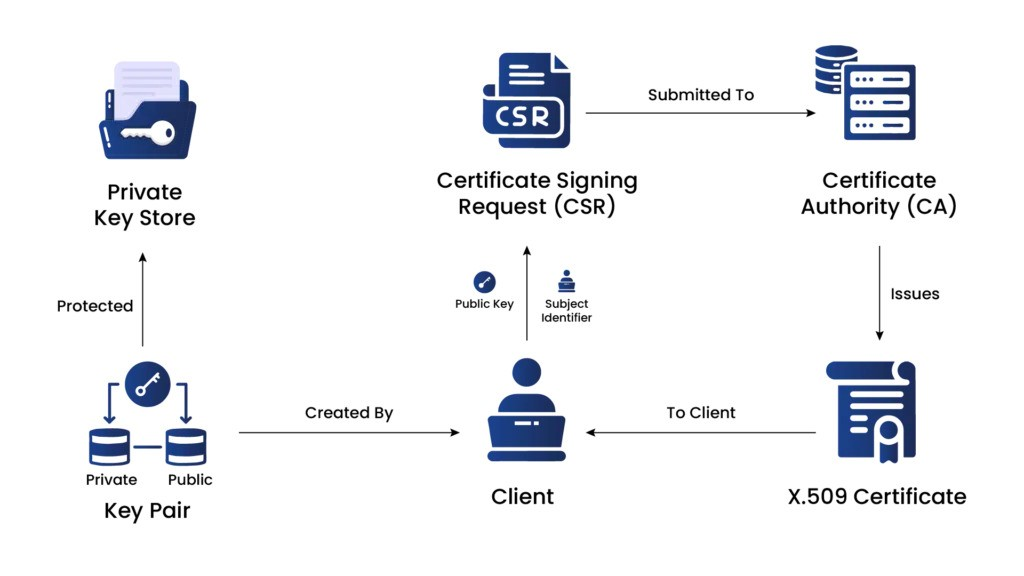
\includegraphics[width=0.8\textwidth]{CertEnr.jpg}
  \caption[Certificate enrollment.]{\label{fig:certenr}Deze afbeelding toont de stappen en componenten in het certificaat uitgave proces.}
\end{figure}

Wanneer een certificaat wordt aangevraagd bij een CA, moet de aanvrager eerst een public en private key genereren. De private key moet onder de controle en eigendom van de aanvrager blijven. In sommige gevallen worden de private keys gegenereerd en veilig bewaart in een Hardware Security Module (HSM). \autocite{SSLcom}
Om de registratie van certificaten te starten, maakt de aanvrager een Certificate Signing Request (CSR) aan. Deze CSR bevat de public key en andere informatie van de aanvrager die in het certificaat zal worden opgenomen, zoals de domeinnaam voor een SSL/TLS certificaat of de aanvrager's e-mail adres voor een S/MIME certificaat.
Daarna wordt de CSR ingedient bij de CA. De CA zal de identiteit van de aanvrager samen met de bijkomende informatie verifiëren. De CA kan verschillende manieren gebruiken om de aanvrager zijn identiteit te verifiëren, zoals e-mail verificatie, domein validatie of manuele validatie van juridische documenten.
Wanneer de CA het verificatie proces heeft voltooid en vaststelt dat de aanvrager legitiem is, zal het digitale certificaat worden uitgegeven. Het certificaat zal de aanvrager zijn public key en bijkomende informatie bevatten, alsook een geldigheidstermijn en de digitale handtekening van de CA.
Het uitgegeven certificaat wordt dan terug gebracht naar de aanvrager, afhankelijk van de CA en het certificaat type zal het certificaat geleverd worden op een verschillende manier zoals via e-mail, een beveiligd portaal of een andere methode.
Na het ontvangen van het certificaat is het aan de aanvrager om het certificaat te installeren op de toepasselijke server of apparaat waar het zal worden gebruikt. Als voorbeeld, een SSL/TLS certificaat wordt geïnstalleerd op een webserver voor een beveiligde connectie naar een website.
Eenmaal het certificaat is geïnstalleerd, kan het gebruikt worden voor protocolen die verantwoordelijk zijn voor beveiligde communicatie. Clients, gebruikers of andere entiteiten die in contact komen met de certificaat eigenaar kunnen de authenticiteit van het certificaat verifiëren aan de hand van de CA zijn digitale handtekening, wat een beveiligde en betrouwbare connectie verzekerd.
Zoals eerder vermeld hebben deze certificaten een geldigheidstermijn (meestal 1 tot 2 jaren). Voor ze vervallen, moet de aanvrager het certificaat vernieuwen via een gelijkaardig proces om het te kunnen blijven gebruiken zonder onderbrekingen. \autocite{EncCon} \break

Het verifiëren van een certificaat om de bepalen of het vertrouwd kan worden is belangrijk voor de veiligheid van de communicatie.
\Textcite{okta} zegt dat tijdens een SSL/TLS handshake, de client het certificaat van de server ontvangt. De client controleert of het certificaat nog niet vervallen is en dat de domeinnaam en IP adres op het certificaat gelijkaardig zijn aan dat van de server. Daarna zal de client kijken of het certificaat correct is ondertekend door een vertrouwde CA.
In de meeste gevallen zal de server certificate niet ondertekend zijn door de root CA die door de client wordt vertrouwd. In plaats van de root CA zal de client 1 of meerdere intermediate CA's vertrouwen zolang als hun ketting van vertrouwen terug leidt naar een root CA die de client vertrouwd.

Voor elke intermediate CA certificate doet de client hetzelfde verificatie proces waarbij de uitgever (issuer) zijn naam overeenkomt met de certificate eigenaar zijn naam van de volgende certificate in de ketting. Ook wordt de digitale signatuur en public key van het certificaat bekeken om te kijken of deze correct is ondertekend.
Dit proces herhaald zichzelf tot de client komt bij een self-signed root CA certificate die de client vertrouwd.
Op dit moment heeft de client dan een cryptografische ketting van vertrouwen gemaakt tot de server en kan de SSL/TLS handshake verder gaan. \break
\begin{figure}
  \centering
  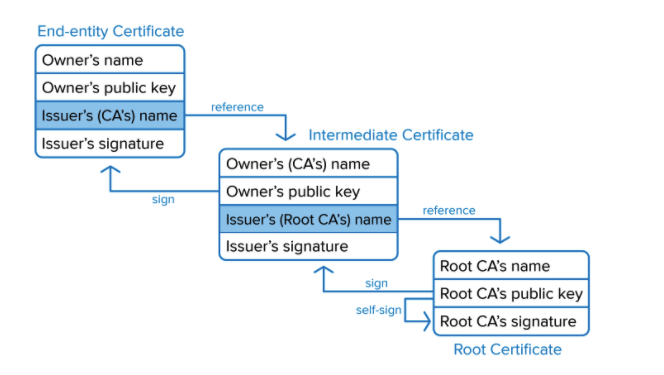
\includegraphics[width=0.8\textwidth]{chainoftrust.png}
  \caption[Chain of trust]{\label{fig:chainoftrust}Deze afbeelding toont de ketting van vertrouwen die de client nakijkt tijdens het verifiëren van een certificaat.}
\end{figure}

Bij dit verificatie proces eindigt de client steeds bij een root CA certificaat die door de client moet worden vertrouwd. Om te bepalen welke root CA's door de client worden vertrouwd bestaan er trust stores.
Een trust store is een collectie van root certificaten die standaard worden vertrouwd door een client en worden beheerd door bedrijven die de client zijn operating system of browser ontwikkelen, zoals Microsoft, Mozilla en Google.
Elke vendor heeft zijn eigen standaarden voor root certificaten maar ze vereisen allemaal dat een uitgevende CA een of meerdere controles ondergaan om hun vertrouwbaarheid, validiteit en conformiteit vast te stellen via de CA/B Forum Baseline Requirements vooraleer ze worden opgenomen in hun trust store. \autocite{Venafi}
Over al de trust stores van deze vendors zijn er heel wat certificaten die niet noodzakelijk zijn. Een studie van \textcite{PerlHenning} toont dat alleen maar 66\% van de certificaten in de trust store van Windows, Linux, MacOS, Firefox, iOS and Android noodzakelijk zijn voor het vertrouwen van websites.
Dit zorgt ervoor dat de overige derde van de root certificaten in de trust stores een potentieel veiligheidsrisico vormen voor de client. \break

Als oplossing hierop kunnen bedrijven het overwegen om deze standaard trust stores af te wijzen. In de plaats daarvan kunnen ze best hun eigen aangepaste, corporate-level trust store maken en gebruik maken van certificate white-listing om te bepalen welke root certificates hierin kunnen opgenomen worden.
Dit helpt bedrijven met het aanvals oppervlak te verkleinen door het limiteren van de hoeveelheid vertrouwde CA's en het markeren van niet-vertrouwde SSL/TLS sessies.
Organisaties kunnen dan deze certificate whitelist en blacklist updaten op een regelmatige basis afhankelijk van benoodigdheden van hun evoluerende business requirements en groeiend CA landschap. \autocite{Venafi} 

Het beheren van deze trust stores kan een uitdaging zijn voor bedrijven, zeker bedrijven met heterogene netwerken (netwerken die clients hebben met verschillende operating systemen en browsers).
\textcite{rfc6024} weerlegt dit door te zeggen dat deze trust anchors (Root CA certificaten) vaak bewaart worden in applicatie-specifieke of OS-specifieke trust stores.
Vaak heeft dan 1 machine een verschillend aantal trust stores die niet gesynchroniseerd zijn met elkaar. \break

De uitdagingen hier zijn dus het vermijden van overbodige vertrouwde root certificaten binnen een netwerk en zijn segmenten afhankelijk van de business requirements en het beheren van deze trust stores over verschillende machines en applicaties. 

\section{\IfLanguageName{dutch}{Verschillende truststores}{Various truststores}}%
\label{sec:Verschillende truststores}

Voor het implementeren van een oplossing voor deze uitdagingen is het van belang om te weten hoe de truststores van de verschillende besturingssystemen en browsers werken en hoe deze kunnen worden beheerd. \break

Windows heeft een truststore die de Trusted Root Certification Authorities store heet.
In de officiële documentatie van Microsoft vermeld \textcite{MStruststore} dat de Trusted Root Certificate Authorities store op een Windows computer via de Microsoft Management Console (MMC) kan worden beheerd door de Certificate Manager snap-in te gebruiken.
De Microsoft Management Console kan worden geopend door het commando \texttt{mmc.exe} uit te voeren in deen Run dialog. In het MCC venster kan men via file -> Add/Remove Snap-in de "Certificates" snap-in toevoegen.
Hierna kan men dan in het MCC venster onder "Certificates (local computer)" -> "Trusted Root Certification Authorities" de lijst van vertrouwde root certificaten bekijken en beheren.
\textcite{MStruststore} vermeld ook dat standaard de Trusted Root Certificate Authorities store geconfigureerd is met een aantal publieke CA's die de vereisten van de Microsoft Root Certificate Program hebben voltooid. \break

Naast de GUI manier van beheren van de truststore, biedt Microsoft ook een manier om het te beheren via de command line aan de hand van het \texttt{certutil} commando.
Certutil.exe is een command-line programma geinstalleerd als onderdeel van de Certitifate Services. Certutil.exe kan gebruikt worden voor het tonen van certificate authority (CA) configuratie informatie, het configureren van Certificate Services en CA componenten te back-uppen en te herstellen.
Dit programma kan ook certificaten, key pairs en certificate chains verifiëren. \autocite{MScertutil}
Om een certificate store te tonen aan de hand van certutil kan het volgende commando worden gebruikt:
\begin{minted}{bash}
  certutil [options] -store [CertificateStoreName [CertId [OutputFile]]]
\end{minted}
Waar CertificateStoreName de naam is van de certificate store, CertId de match token is van het certificaat en OutputFile de naam is van het bestand waarin de overeenkomende certificaten worden opgeslagen. \autocite{MScertutil}

Om een certificaat toe te voegen aan een certificate store kan het volgende commando worden gebruikt:
\begin{minted}{bash}
  certutil [options] -addstore CertificateStoreName InFile
\end{minted}
Waar CertificateStoreName de naam is van de certificate store en InFile de certificate file is die moet worden toegevoegd. \autocite{MScertutil} \break

Linux heeft niet zoals Windows één centrale trust store. In plaats daarvan heeft Linux verschillende trust stores die afhankelijk zijn van de applicatie of fr distributie van Linux.

Binnen Ubuntu Server moet een certificaat in PEM formaat staan vooraleer het kan worden toegevoegd aan de trust store.
Om een PEM-geformatteerd root CA certificaat met als voorbeeld naam "local-ca.crt" te installeren in de trust store van Ubuntu Server kan het volgende commando worden gebruikt:
\begin{minted}{bash}
  sudo apt-get install -y ca-certificates
  sudo cp local-ca.crt /usr/local/share/ca-certificates
  sudo update-ca-certificates
\end{minted}

Het is hierbij belangrijk dat het certificaat bestand de extensie .crt heeft anders zal het niet worden verwerkt.

De trust store (die gegenereerd wordt door update-ca-certificates) is te vinden op de volgende locaties:
\begin{itemize}
  \item Als een file (PEM bundel) in /etc/ssl/certs/ca-certificates.crt
  \item Als een OpenSSL-compatibele certificaat directory in /etc/ssl/certs/ca-certificates.pem
\end{itemize} \autocite{UbunTruststore}
\break

Red Hat Enterprise Linux (RHEL) heeft een andere manier van het beheren van de trust store. RHEL biedt de Shared System Certificates aan.
De Shared System Certificates storage laat NSS, GnuTLS, OpenSSL en Java toe om een standaard bron te delen voor het ophalen van systeem certificate anchors en black list informatie.
Standaard bevat de truststore de Mozilla CA list, die positieve en negatieve trust informatie bevat. Het systeem laat toe om de Mozilla CA lijst aan te passen of om een andere CA lijst te gebruiken. \autocite{RHELtruststore} \break

In Red Hat Enterprise Linux 7 is de systeem-brede truststore te vinden in de directories /etc/pki/ca-trust/ en /usr/share/pki/ca-trust-source/ . De trust settings in /usr/share/pki/ca-trust-source/ worden behandeld met een lagere prioriteit dan de settings in /etc/pki/ca-trust/ .
Certificaat bestanden worden anders behandeld afhankelijk van de subdirectory waarin ze worden geplaatst:
\begin{itemize}
  \item /usr/share/pki/ca-trust-source/anchors/ of /etc/pki/ca-trust/source/anchors/ : voor trust anchors.
  \item /usr/share/pki/ca-trust-source/blacklist/ of /etc/pki/ca-trust/source/blacklist/ : voor niet vertrouwde certificaten.
  \item /usr/share/pki/ca-trust-source/ of /etc/pki/ca-trust/source/ : voor certificaten in de extended BEGIN TRUSTED bestandsformaat.
\end{itemize} \autocite{RHELtruststore}

Om een certificaat in de simpele PEM of DER bestandsformaten aan de lijst van vertrouwde CA's op het systeem toe te voegen, kan je simpelweg het certificaat bestand kopiëren naar de /usr/share/pki/ca-trust-source/anchors/ of /etc/pki/ca-trust/source/anchors/ directory. Om de systeem-brede truststore te updaten ka je het update-ca-trust commando gebruiken zoals volgt:
\begin{minted}{bash}
  cp ~/certificate-trust-examples/Cert-trust-test-ca.pem /usr/share/pki/ca-trust-source/anchors/
  update-ca-trust
\end{minted} 

Om de trust anchors op te lijsten, toe te voegen, veranderen of verwijderen kan het 'trust' commando gebruikt worden.
Voor het oplijsten van de trust anchors wordt 'trust list' gebruikt.
Een trust anchor opslaan in de trust store kan met het 'trust anchor' sub-commando en het specifiëren van het pad (vb.: 'path.to') naar het certificaat bestand, zoals volgt:
\begin{minted}{bash}
  trust anchor path.to/certificate.crt
\end{minted} 
Om een trust anchor te verwijderen kan een pad naar het certificaat of ID van het certificaat gebruikt worden:
\begin{minted}{bash}
  trust anchor --remove path.to/certificate.crt
  trust anchor --remove "pkcs11:id=%AA%BB%CC%DD%EE;type=cert"
\end{minted} 
\autocite{RHELtruststore} \break

Applicaties kunnen ook hun eigen trust store hebben. Een voorbeeld hiervan is Mozilla Firefox. Firefox maakt gebruik van de NSS (Network Security Services) library voor het beheren van de trust store.
De Network Security Services (NSS) library is een set van libraries ontwikkeld om cross-platform ontwikkeling van veilige client en server applicaties te ondersteunen. De libraries ondersteunen SSL v3, TLS, PKCS #5, PKCS #7, PKCS #11, PKCS #12, S/MIME, X.509 v3 certificaten en andere security standaarden. \autocite{FirefoxNNS}
Firefox geeft bij initiatie een string met pad naar de directory waar NSS de security en configuratie data mag opslaan. NSS slaat 3 bestanden op in die directory:
\begin{itemize}
  \item cert8.db: slaat publiek toegankelijke objecten op (Certificaten, CRL's, S/MIME records).
  \item key3.db: slaat private keys op.
  \item secmod.db: slaat de PKCS#11 module configuratie op.
\end{itemize}
Als in deze directory grote security objecten zitten (zoals grote CRL's), zal NSS deze opslaan in bestanden in subdirectories genaamd 'cert8.dir'.
In het geval dat cert8.db en/of key3.db niet bestaan, zal NSS de data lezen van oudere versies vand eze databases (bv.: cert7.db, cert6.db,...) en zal deze data gebruiken om een nieuwe cert8.db en key3.db te maken. \autocite{MozillaWiki}

Ook beweert \textcite{MozillaCA} dat standaard Firefox op Windows, MacOS en Android zal zoeken en gebruik maken van de third-party CA's die zijn opgenomen in de operating system zijn trust store.
Firefox kan geconfigureerd worden om automatisch te zoeken naar CA's die in de Windows certificate store zijn toegevoegd door een gebruiker of administrator. Dit kan gedaan worden door de \texttt{security.enterprise_roots.enabled} optie in te stellen op 'true' in de config van Firefox.
Firefox zal dan de HKLM/SOFTWARE/Microsoft/SystemCertificates (Het pad dat overeenstemt met de API flag CERT\_SYSTEM\_STORE\_LOCAL\_MACHINE) registry directory inspecteren voor CA's die vertrouwd worden om certiifcaten uit te geven voor TLS web server authenticatie. \autocite{MozillaCA}
Ook wordt er gekeken naar de volgende andere locaties:
\begin{itemize}
  \item HKLM/SOFTWARE/Policies/Microsoft/SystemCertificates/Root/Certificates (pad in API flag CERT\_SYSTEM\_STORE\_LOCAL\_MACHINE\_GROUP\_POLICY)
  \item HKLM/SOFTWARE/Microsoft/EnterpriseCertificates/Root/Certificates (pad in API flag CERT\_SYSTEM\_STORE\_LOCAL\_MACHINE\_ENTERPRISE)
\end{itemize} \autocite{MozillaCA}

\textcite{MozillaCA} voorziet ook dat enterprise policies kunnen gebruikt worden voor het toevoegen van CA certificaten in Firefox.
De 'ImportEnterpriseRoots' key op 'true' zetten, zorgt ervoor dat Firefox root certificaten zal vertrouwen.
De 'Install' key zoekt standaard naar certificaten in de onderstaande locaties. Er kan ook een specifiek pad worden opgegeven. Als Firefox daar geen certificaten vindt zal het de standaard directories bekijken:
\begin{itemize}
  \item Windows
  \begin{itemize}
    \item \%USERPROFILE\%\symbol{92}AppData\symbol{92}Local\symbol{92}Mozilla\symbol{92}Certificates 
    \item \%USERPROFILE\%\symbol{92}AppData\symbol{92}Roaming\symbol{92}Mozilla\symbol{92}Certificates
  \end{itemize}

  \item macOS
  \begin{itemize}
    \item /Library/Application Support/Mozilla/Certificates 
    \item ~/Library/Application Support/Mozilla/Certificates 
  \end{itemize}

  \item Linux 
  \begin{itemize}
    \item /usr/lib/mozilla/certificates 
    \item /usr/lib64/mozilla/certificates 
  \end{itemize}
\end{itemize} \autocite{MozillaCA} \break

\section{\IfLanguageName{dutch}{Bestaande tools}{Existing tools}}%
\label{sec:Bestaande tools}

Er bestaan verschillende gratis tools die kunnen helpen met het beheren van truststores over verschillende machines en applicaties.
Deze tools zijn niet ontwikkeld specifiek voor het beheren van truststores maar bieden functionaliteiten aan voor het beheren van end-points hun configuratie.
Voor Windows bestaat Microsoft System Center Configuration Manager (SCCM).

\textcite{ConfigMan} zegt dat Configuration Manager deel uitmaakt van de Microsoft Intune familie van producten. De Microsoft Intune familie van producten is een geïntegreerde oplossing voor het beheren van al jouw apparaten.
Configuration Manager vebreed en werkt samen met vele Microsoft technologieëen en oplossing zoals onder andere Certificate Services.

Een meer algemene oplossing die werkt voor beide Windows en Linux is Ansible.
Ansible is een open-source IT automation engine die provisioning, configuratie management, applicatie deployment, orkestratie en vele andere IT taken automatiseert.
Ansible kan gratis worden gebruikt en het project profiteert van de ervanging en intelligentie van zijn duizende gebruikers. \autocite{Ansible}

Ansible zijn grootste sterkte is eenvoud. Het heeft ook een sterke focus op beveiliging en betrouwbaarheid, met zo weinig mogelijk bewegende delen. Het gebruikt OpenSSH voor transport (met andere transport en pull modes beschikbaar als alternatieven), en gebruikt leesbare taal die ontworpen is om snel aan de start te kunnen gaan zonder enige training.
Red Hat Ansible Automation Platform is een abbonement gebaseerde oplossing die bouwt op de basis van Ansible met een aantal ondernemingsgerichte functionaliteiten.
Beide community Ansible en Ansible Automation Platform zijn gebouwt op het concept van een control node en een managed node. Ansible wordt gebruikt op de control node waar bijvoorbeeld een gebruiker een ansible-playbook command uitvoert. Managed nodes zijn de apparaten die worden geautomatiseerd zoals bijvoorbeeld een Windows server.
Voor Linux en Windows te automatiseren, connecteert Ansible met de managed nodes en verstuurt het kleine programma's genaamd Andisble modules uit. Deze programma's zijn geschreven als bronmodellen van de gewenste staat van het systeem. Ansible voert dan deze modules uit (standaard over SSH), en verwijdert ze na ze voltooien.
Deze modules zijn ontworpen om idempotent te zijn waar mogelijk, zodanig ze alleen een aanpassing uitvoeren op een systeem als dat nodig is. \autocite{AnisbleHow} \break

Een andere tool die mogelijks kan helpen is Open Source Puppet.
Puppet is een open source configuratie management tool geproduceert door Puppet Labs. Er kunnen systeem configuraties gedefinieerd worden aan de hand van Puppet's declaratieve taal en deze configuraties kunnen dan opgeslagen worden in bestanden genaamd Puppet Manifests.
Puppet kan standalone op een systeem draaien of in een agent/master configuratie. Met standalone Puppet draaien systemen het programma lokaal om hun eigen configuraties aan te passen. Met agent/master Puppet beheert een centrale Puppet master server of servers meerdere systemen die de Puppet agent draaien.
Bij beide implementaties worden Puppet manifests gebruikt om systeem configuraties naar de verwachte staat te brengen. Daarnaast bestaat er ook nog een commerciële versie van Puppet genaamd Puppet Enterprise. \autocite{Puppet} \break

Naast Ansible en Puppet bestaan er ook nog andere tools zoals Saltstack en Chef.
Gebouwt op Python, is Salt een event-driven automatiseringstool en framework dat is ontworpen om complexe IT systemen te deployeren, configureren en beheren. Salt kan gebruikt worden voor veel voorkomende administratie taken te automatiseren en te verzekeren dat alle componenten van je infrastructuur operationeel zijn in de verwachte staat.
Salt heeft vele mogelijke gebruiksdoeleinden, zoals configuratie beheer, wat als volgt inhoud:
\begin{itemize}
  \item Het beheren van het deployeren van besturingssystemen en hun configuratie.
  \item Het installeren en configureren van software applicaties en diensten.
  \item Het beheren servers, virtuele machines, containers, databases, web servers, netwerk apparaten en meer.
  \item Verzekeren dat de configuratie consistent is en het vermijden van drift.
\end{itemize}

Salt maakt het mogelijk om applicaties te implementeren en beheren die gebruik maken van elke technologiestack die op bijna elk besturingssysteem draait, inclusief verschilllende soorten netwerkapparaten zoals switches en routers van verschillende leveranciers.
Daarnaast kan het ook gebruikt worden voor het automatiseren en orkestreren van routine IT processen zoals veel voorkomende noodzakelijke taken voor geplande server downtime of het upgraden van besturingssystemen en applicaties. 
Ook kan Salt gebruikt worden om een zelfbewuste, zelf herstellende systemen te maken die automatisch kunnen reageren op uitvallingen, veel voorkomende administratie problemen of andere belangrijke gebeurtenissen. \autocite{Saltstack} \break

\textcite{Chef} noemt Chef een automation company. Vandaag biedt Chef automatiseringsoplossingen voor beide infrasctructuur en applicaties van ontwikkeling tot productie.
Chef Infra automatiseert hoe infrastructuur is geconfigureerd, gedeployed en beheerd doorheen het netwerk, ongeacht de grootte.

Chef Workstation maakt het mogelijk om 'cookbooks' te schrijven en je infrastructuur te beheren. Chef Workstation hoort te draaien op de machine die je dagelijks gebruikt, ongeacht of deze Windows, Linux of MacOS draait.
Eenmaal het ontwikkelen van je code gedaan is op je workstation, dan kan je deze code uploaden naar de CHef Infra Server. De Chef Infra Server is een centrale opslagplaats voor je configuratie data. Het slaat cookbooks, policies en metadata van elk systeem op. Het communiceren met de Chef Infra Server vanaf een workstation kan via het 'knife' commando.
Chef Infra Clients contacteren deze Chef Infra Server periodiek om de laatste cookbooks op te halen. Als de huidige staat van de node niet overeenstemt met wat de cookbook beschrijft, zal de Chef Infra Client de cookbook instrucites uitvoeren. \autocite{Chef} \break

\section{\IfLanguageName{dutch}{Infrastructuur studie}{Infrastructure study}}%
\label{sec:Infrastructuur studie}

Voor een realistisch beeld te scheppen van een bedrijfsomgeving, zal er gekeken worden naar resultaten van meerdere vragenlijsten en enquêtes die het marktaandeel van verschillende technologieëen onderzoeken. \break

\textcite{NetcraftSurvey} publiceert maandelijks een web server survey waarin ze de marktaandelen van web servers onderzoeken, uit de resultaten van de survey van januari 2025 blijkt Nginx het grootste marktaandeel te hebben binnen alle onderzochte sites met 19,60\% alsook alle onderzochte actieve sites met 18,89\%.
Naast Nginx heeft Apache het tweede grootste marktaandeel met 16,96\% van alle onderzochte sites en 17,24\% van alle actieve sites. \break

Binnen de Stack Overflow developer survey van 2024 kan er ook gekeken worden naar veel gebruikte technologieëen binnen de professionele wereld.
In de resultaten kan er gekeken worden naar welke van de eerder vermelde tools het meest gebruikt worden in de professionele wereld. \autocite{StackOverflowSurvey} rapporteert onder overige tools dat Ansible gebruikt wordt door 8,1\% van de ondervraagde professionele developers, Pupper door 1,1\% en Chef door 0,7\%. \break

Binnen de resultaten van de Stack Overflow survey kan er ook gekeken worden naar de meest gebruikte databases. Uit deze resultaten blijkt dat PostgreSQL de meest gebruikte database is met 51,9\% van de ondervraagde professionele developers die het gebruiken. MySQL is de tweede meest gebruikte database met 39,4\% van de ondervraagde professionele developers die het gebruiken. \autocite{StackOverflowSurvey} \break

Het bepalen welke DNS server technologie het meest gebruikt wordt binnen bedrijven is moeilijk omdat dit geen publiek beschikbare data is. Hier zal BIND gekozen worden, volgens \textcite{Bind9} is BIND 9 de eerste, oudste en meest gebruikte oplossing waarmee netwerk engineers al meer bekend zijn dan met andere systemen. \break

\textcite{SecSpMail} publiceert ook rapporten op verschillende technologieëen. Een van deze rapporten bestudeert alle zichtbare mailservers op het internet en kijkt naar welke onderliggende software ze gebruiken. Uit de resultaten van Maart 2025 blijkt dat Exim de meest gebruikte mailserversoftware is met 55,05\% en Postfix de tweede meest gebruikte met 38,52\%. \break

Deze informatie zal gebruikt worden voor het bepalen van de gebruikte technologieëen binnen de proof-of-concept virtuele omgeving.
%\begin{figure}
%  \centering
%  \includegraphics[width=0.8\textwidth]{grail.jpg}
%  \caption[Voorbeeld figuur.]{\label{fig:grail}Voorbeeld van invoegen van een figuur. Zorg altijd voor een uitgebreid bijschrift dat de figuur volledig beschrijft zonder in de tekst te moeten gaan zoeken. Vergeet ook je bronvermelding niet!}
%\end{figure}

%\begin{listing}
%  \begin{minted}{python}
%    import pandas as pd
%    import seaborn as sns
%
%    penguins = sns.load_dataset('penguins')
%    sns.relplot(data=penguins, x="flipper_length_mm", y="bill_length_mm", hue="species")
%  \end{minted}
%  \caption[Voorbeeld codefragment]{Voorbeeld van het invoegen van een codefragment.}
%\end{listing}

%\lipsum[7-20]

%\begin{table}
%  \centering
%  \begin{tabular}{lcr}
%    \toprule
%    \textbf{Kolom 1} & \textbf{Kolom 2} & \textbf{Kolom 3} \\
%    $\alpha$         & $\beta$          & $\gamma$         \\
%    \midrule
%    A                & 10.230           & a                \\
%    B                & 45.678           & b                \\
%    C                & 99.987           & c                \\
%    \bottomrule
%  \end{tabular}
%  \caption[Voorbeeld tabel]{\label{tab:example}Voorbeeld van een tabel.}
%\end{table}


%%=============================================================================
%% Methodologie
%%=============================================================================

\chapter{\IfLanguageName{dutch}{Methodologie}{Methodology}}%
\label{ch:methodologie}

%% TODO: In dit hoofstuk geef je een korte toelichting over hoe je te werk bent
%% gegaan. Verdeel je onderzoek in grote fasen, en licht in elke fase toe wat
%% de doelstelling was, welke deliverables daar uit gekomen zijn, en welke
%% onderzoeksmethoden je daarbij toegepast hebt. Verantwoord waarom je
%% op deze manier te werk gegaan bent.
%% 
%% Voorbeelden van zulke fasen zijn: literatuurstudie, opstellen van een
%% requirements-analyse, opstellen long-list (bij vergelijkende studie),
%% selectie van geschikte tools (bij vergelijkende studie, "short-list"),
%% opzetten testopstelling/PoC, uitvoeren testen en verzamelen
%% van resultaten, analyse van resultaten, ...
%%
%% !!!!! LET OP !!!!!
%%
%% Het is uitdrukkelijk NIET de bedoeling dat je het grootste deel van de corpus
%% van je bachelorproef in dit hoofstuk verwerkt! Dit hoofdstuk is eerder een
%% kort overzicht van je plan van aanpak.
%%
%% Maak voor elke fase (behalve het literatuuronderzoek) een NIEUW HOOFDSTUK aan
%% en geef het een gepaste titel.

Het onderzoek naar centrale truststorebeheer zal opgedeeld worden in drie fases: een literatuurstudie, praktijkstudie en uiteindelijke rapportage en oplevering.

In de eerste anderhalve maand zal de eerste fase van het onderzoek uitgevoerd worden, de literatuurstudie.

Het doel in deze fase is om een diepgaand begrip te krijgen over trust management, certificaatbeheer en de verschillende aanpakken bij truststorebeheer.

In deze literatuurstudie zal er gekeken worden naar de bestaande theorieën, technologieën en andere tools die momenteel worden gebruikt in praktijk.

Ook zal er gekeken worden naar de uitdagingen van trust management in een omgeving met netwerksegmentatie en diverse applicaties en besturingssystemen.

Doorheen deze fase zal er periodiek overleg zijn met de co-promotor om de voortgang te bespreken en een mogelijkse oplossing te kiezen die verder kan worden uitgewerkt in de praktijkstudie.

De info die verkregen wordt in deze literatuurstudie zal de basis leggen voor de volgende fase van dit onderzoek: de praktijkstudie.

Deze fase zou starten halverwege maart en loopt tot eind april met een duur van 6 weken. Deze praktijkstudie opgedeeld in 3 delen.

het ontwerpen van een virtuele omgeving, de implementatie van het centraal truststorebeheer en de evaluatie van de oplossing.

In de eerste stap zal er weer worden gekeken naar veel gebruikte software en besturingssystemen binnen bedrijven om zo een realistische infrastructuur te creëren.

Ook wordt er een certificate authority (CA) opgezet om het beheer van certificaten en een interne private PKI te simuleren.

Deze virtuele omgeving zal worden opgezet binnen GNS3, een netwerkemulator die het mogelijk maakt om complexe netwerken te simuleren.

De tweede stap, de implementatie van centraal truststorebeheer, begint eind maart en duurt drie weken.

In deze fase wordt een gecentraliseerde oplossing voor truststorebeheer opgezet. Dit gebeurt door middel van de tools die gekozen werden samen met de co-promotor in de literatuurstudie in combinatie met eventuele zelfgeschreven scripts voor het certificaatbeheer.

Het doel hier is dat bij het genereren of updaten van een nieuw root certificaat, de truststores op elk systeem in het netwerk en zijn segmenten consistent zijn. Ook zullen er veiligheidscontroles geïmplementeerd worden, zoals het monitoren voor ongeldige of verlopen certificaten.

Na de implementatie volgt de derde stap van de praktijkstudie, die bestaat uit de evaluatie en validatie van de oplossing.

Deze fase begint begin halfweg april en duurt 2 weken.

De centrale vraag is hoe kwaliteitsvol de oplossing is en of deze voldoet aan de verwachtingen.

Er worden testcases opgesteld om veelvoorkomende uitdagingen te simuleren, zoals het herroepen van een rootcertificaat of het omgaan met verlopen certificaten.

Ook wordt de schaalbaarheid en efficiëntie van de oplossing getest.

Bij de schaalbaarheid zal er gekeken worden naar hoe de oplossing omgaat met het veranderen of uitbreiden van het netwerk. Bij de efficiëntie zal er gekeken worden naar hoe snel aanpassingen van certificaten binnen de centrale truststore verspreid worden binnen het netwerk zonder het verstoren van andere diensten.

Als laatste fase van dit onderzoek zal er een rapportage gemaakt worden. Dit zal gebeuren in het begin van mei met een tijdsduur van 4 weken. De rapportage zal de ontwerpkeuzes en oplossing binenn de PoC beschrijven alsook de evaluatie en resultaten van deze oplossing.

Op basis van de bevindingen worden dan conclusies en aanbevelingen geformuleerd voor de implementatie van centraal truststorebeheer alsook welke aspecten mogelijks verder onderzoek vereisen.



\chapter{\IfLanguageName{dutch}{Proof-of-concept}{Proof-of-concept}}%
\label{ch:proof-of-concept}
\section{\IfLanguageName{dutch}{Virtuele omgeving}{Virtual environment}}%
\label{sec:Virtuele_omgeving}

Voor het opzetten van een oplossing en deze te kunnen testen en evalueren, is er een virtuele omgeving opgezet.
Deze virtuele omgeving is opgezet in GNS3, een netwerkemulator die het mogelijk maakt om netwerkapparatuur alsook virtuele machines te simuleren.
Binnen deze virtuele omgeving zal er aan netwerksegmentatie gedaan worden, het netwerk zal opgedeelde worden in 3 segmenten: een Admin, DMZ en employee segment.
Binnen het Admin segment zullen grotendeels van de servers staan alsook een workstation, in het DMZ segment zal er 1 server staan en in het employee segment zullen de werkstations staan.
Deze segmentatie bestaat met als doel om het aantal vertrouwde root certificaten te beperken tot de benodigdheden van de verschillende segmenten, zo worden er minder root certificaten vertrouwd door de verschillende segmenten wat tot lagere security risico's leidt.
Binnen het Admin segment staan er 4 servers, "Windowsserver", "Database", "CA" en "Vault" alsook is hier een workstation "Admin-client". Het DMZ segment heeft een server "Webserver" en het employee segment heeft 1 workstation "Employee-client". \\

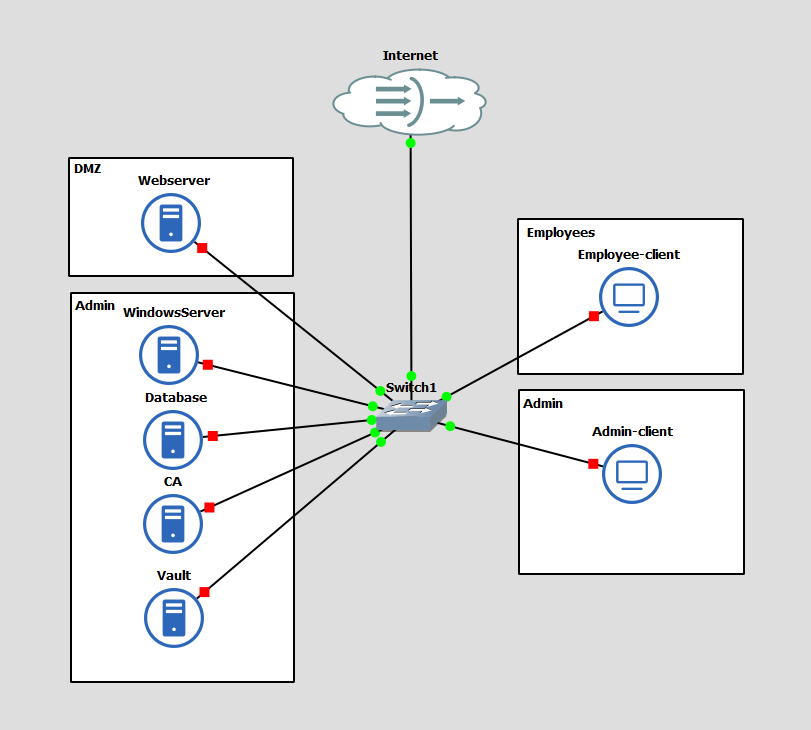
\includegraphics[width=1\textwidth]{Architectuurplan.png}

\subsection{\IfLanguageName{dutch}{Webserver}{Webserver}}
\label{subsec:Webserver}

De webserver draait op Ubuntu 22.04 en heeft een Nginx webserver draaien met een certificaat dat ondertekend werd door de CA server van binnen deze virtuele omgeving.
Het doel van deze webserver is om de functionaliteit van het aanpassen van de truststore te testen, als een end-point de webpagina kan bereiken zonder waarschuwing via het https protocol, dan betekent dat de server "CA" zijn root certificaat aanwezig is in de end-point zijn truststore.

\subsection{\IfLanguageName{dutch}{Windows server}{Windows server}}
\label{subsec:Windows_server}

Deze server draait Windows Server 2022 en is de domein controller van de virtuele omgeving. Het domein is "Bachelorproef.local" en de server heeft een Active Directory (AD) opgezet. De Active Directory bevat 2 logins voor de Windows clients "Employee1" en "Admin1". Binnen de AD zal elke Windows client die het netwerk betreedt automatisch gestoken worden. 
Deze clients worden manueel in de juiste organisational unit (OU) gestoken. In dit geval zijn dit de OU "Employee" en "Admin".

\subsection{\IfLanguageName{dutch}{CA}{CA}}
\label{subsec:CA}

De CA server draait een Almalinux 8.8 image en is een Certificate Authority (CA). Het root certificaat is gemaakt met OpenSSL en is ondertekend door de CA zelf. Zoals eerder vermeld is er een leaf certificaat aangemaakt en ondertekend voor de webserver.

\subsection{\IfLanguageName{dutch}{Vault}{Vault}}
\label{subsec:Vault}

De Vault server draait ook Ubuntu 22.04 en heeft een Hashicorp Vault server draaien. Deze vault server zal gebruikt worden om de root certificaten op een centrale plaats op te slaan.

\subsection{\IfLanguageName{dutch}{Employee-client}{Employee-client}}
\label{subsec:Employee-client}

Deze Windows client draait Windows 11, en bevindt zich in het Employee netwerksegment. Deze client maakt deel uit van het domein "Bachelorproef.local" en is ook lid van de OU "Employee".

\subsection{\IfLanguageName{dutch}{Admin-client}{Admin-client}}
\label{subsec:Admin-client}

Deze Windows client draait ook Windows 11 en bevindt zich in het Admin netwerksegment. Deze client maakt ook deel uit van het domein "Bachelorproef.local" en is ook lid van de OU "Admin".

\section{\IfLanguageName{dutch}{Eerste oplossing}{First solution}}%
\label{sec:Eerste_oplossing}
\subsection{\IfLanguageName{dutch}{Oplossing voor Windows end-points door middel van GPO's met root certificaten}{Solution for Windows end-points using GPOs with root certificates}}
\label{subsec:Oplossing_voor_Windows_end-points_door_middel_van_GPOs_met_root_certificaten}
Om Windows clients hun truststores centraal te kunnen beheren, kan er simpelweg een GPO (Group Policy Object) aangemaakt worden die root certificaten bevat en deze kan dan toegepast worden op een OU binnen de Active Directory.
Er kan dus een GPO aangemaakt worden per OU (in dit geval de 3 OU's voor de 3 netwerksegmenten) die elk de juiste root certificaten bevatten.
Voor deze proof of concept zal er een verzameling van root certificaten opgeslagen worden in een directory op de Windows server, deze directory zal 3 subdirectories bevatten voor elk netwerksegment. De root certificaten die in deze subdirectories staan zijn de root certificaten die de clients in dat netwerksegment moeten vertrouwen.
De GPO's zullen dan de root certificaten uit deze subdirectories halen en deze toevoegen aan de truststore van de clients in dat netwerksegment.
De GPO's kunnen als volgt aangemaakt worden:
\begin{itemize}
    \item Open de Group Policy Management Console (GPMC) op de Windows server.
    \item Maak een nieuwe GPO aan door met de rechtermuisknop op de OU te klikken en "Create a GPO in this domain, and Link it here" te selecteren.
    \item Geef de GPO een naam, bijvoorbeeld "Employee-certificates".
    \item Klik met de rechtermuisknop op de GPO en selecteer "Edit".
    \item Ga naar Computer Configuration > Policies > Windows Settings > Security Settings > Public Key Policies > Trusted Root Certification Authorities.
    \item Klik met de rechtermuisknop en selecteer "Import".
    \item Volg de wizard om het root certificaat te importeren vanuit de directory op de Windows server.
    \item Herhaal deze stappen voor de andere OU's en root certificaten.
\end{itemize}

De GPO's kunnen dan toegepast worden, dit kan door met de rechtermuisknop op de OU te klikken en "Link an Existing GPO" te selecteren. Selecteer dan de GPO die je wilt toepassen op de OU. \\

Op de clients kan je dan de GPO's toepassen door het volgende commando uit te voeren in de command prompt:
\begin{minted}{powershell}
    gpupdate /force
\end{minted}
Ook kan de GPO toegepast worden door de clients opnieuw op te starten. \\

\subsection{\IfLanguageName{dutch}{Oplossing voor Linux end-points met Ansible}{Solution for Linux end-points using Ansible}}
\label{subsec:Oplossing_voor_Linux_end-points_met_Ansible}
Om het probleem van het centraal beheren van de root certificaten op te lossen, kan er een Ansible playbook gemaakt worden dat root certificaten kan toevoegen aan de truststores van de Linux systemen.
De CA server zal in deze proof-of-concept ook de Ansible control server zijn. Dit is de server die de Ansible playbooks zal uitvoeren op de end-points.
Hiervoor is een inventory bestand nodig dat de IP adressen van de end-points bevat alsook de locatie van de key en gebruiker die gebruikt zal worden voor de SSH verbinding. Dit bestand voor deze omgeving ziet er als volgt uit:
\begin{minted}{yaml}
    [DMZ]
    web ansible\_host=bpweb.bachelorproef.local ansible\_user=ubuntu ansible\_ssh\_private\_key\_file=/home/almalinux/.ssh/id\_rsa

    [Admin]
    db ansible\_host=db.bachelorproef.local ansible\_user=almalinux ansible\_ssh\_private\_key\_file=/home/almalinux/.ssh/id\_rsa
    ca ansible\_host=ca.bachelorproef.local ansible\_user=almalinux ansible\_ssh\_private\_key\_file=/home/almalinux/.ssh/id\_rsa
\end{minted}

Net zoals bij de Windows server zal er een directory aangemaakt worden op de server "CA" die subdirectories bevat voor elk netwerksegment. Deze subdirectories bevatten de root certificaten die de end-points in dat netwerksegment moeten vertrouwen.
Met deze bestanden en directories kan er een Ansible playbook gemaakt worden dat de root certificaten uit de juiste subdirectory haalt en toevoegt aan de truststore van de end-points. Dit kan gedaan worden met het volgende Ansible playbook:
\begin{minted}{yaml}
    - name: Installeer en vervang alle root certificaten per groep
        hosts: all
        become: true
        vars:
        cert\_source\_dir: >-
            {{ '/home/almalinux/Ansible/DMZ' if 'DMZ' in group\_names else '/home/almalinux/Ansible/Admin' }}
        dest\_cert\_dir: >-
            {{ '/usr/local/share/ca-certificates' if ansible\_os\_family == "Debian" else '/etc/pki/ca-trust/source/anchors' }}
        update\_command: >-
            {{ 'update-ca-certificates' if ansible\_os\_family == "Debian" else 'update-ca-trust extract' }}
    
        tasks:
    
        ### BACKUP STANDAARD TRUSTSTORE ###
        - name: Maak back-up van standaard truststore op Debian
            when: ansible\_os\_family == "Debian"
            command: >
            tar czf /root/debian-ca-certificates-backup.tar.gz /usr/share/ca-certificates /etc/ssl/certs
    
        - name: Maak back-up van standaard truststore op RedHat
            when: ansible\_os\_family == "RedHat"
            command: >
            tar czf /root/redhat-ca-certificates-backup.tar.gz /etc/pki/ca-trust
    
        ### VERWIJDER STANDAARD CERTIFICATEN ###
        - name: Ledig standaart truststore op Debian
            when: ansible\_os\_family == "Debian"
            file:
            path: "{{ item }}"
            state: absent
            loop:
            - /usr/share/ca-certificates/mozilla
            - /etc/ssl/certs/ca-certificates.crt
    
        - name: Ledig standaart truststore op RedHat
            when: ansible\_os\_family == "RedHat"
            shell: rm -f /etc/pki/ca-trust/source/anchors/*
            args:
            warn: false
    
        ### CERTIFICATEN INSTALLEREN ###
        - name: Zoek alle certificaten in groepsspecifieke map
            find:
            paths: "{{ cert\_source\_dir }}"
            patterns: "*.crt"
            register: certs\_to\_install
    
        - name: Kopieer certificaten naar truststore directory
            copy:
            src: "{{ item.path }}"
            dest: "{{ dest\_cert\_dir }}/{{ item.path | basename }}"
            owner: root
            group: root
            mode: '0644'
            loop: "{{ certs\_to\_install.files }}"
            when: certs\_to\_install.matched > 0
    
        ### TRUST STORE UPDATEN ###
        - name: Update systeem truststore
            command: "{{ update\_command }}"
    
        ### VERIFICATIE ###
        - name: Bevestiging
            debug:
            msg: "Alle root certificaten zijn geïnstalleerd en de truststore is bijgewerkt!" 
\end{minted}

De playbook begint met het maken van een back-up van de standaard out-of-the-box truststores, dit is belangrijk aangezien de tweede stap deze zal leegmaken. Moest een belangrijke root certificaat ontbreken na het uitvoeren van de playbook, kan deze teruggezet worden met de back-up.
Deze playbook kijkt vervolgens naar welke groep de end-point inzit om zo de certificaten uit de directory met dezelfde naam te halen, daarna worden de certificaten gekopieerd naar de directory op de end-points die de truststores bekijken en tenslotte wordt de truststore geüpdatet met het juiste commando. 
Deze playbook bepaalt de bestemmingsdirectory en het update commando op basis van de 'OS family' van de end-point.
In dit geval is dit Debian of Red Hat, voor andere OS families zouden deze nog manueel moeten worden toegevoegd samen met de juiste commando's en directories. \\

Om het voorgaande Ansible playbook uit te voeren, kan er gebruik gemaakt worden van de volgende commando's:
\begin{minted}{bash}
    ansible-playbook -i inventory playbook.yml
\end{minted}

Waarbij "inventory" het inventory bestand is dat de IP adressen van de end-points bevat en "playbook.yml" het Ansible playbook is dat de root certificaten toevoegt aan de truststores van de end-points. \\

\subsection{\IfLanguageName{dutch}{Pro's en Con's van de eerste oplossing}{Pro's and Con's of the first solution}}
\label{subsec:Pros_en_Cons_van_de_eerste_oplossing}
\begin{itemize}
    \item Pro's:
    \begin{itemize}
        \item De root certificaten kunnen eenvoudig beheerd worden.
        \item Geen nodige installatie van extra software op de end-points.
        \item End-points ondervinden geen hinder van de installatie van de root certificaten.
        \item Er zijn weinig points of failure aangezien de oplossing geen bijkomende servers of software nodig heeft.
    \end{itemize}
    \item Con's:
    \begin{itemize}
        \item De GPO's passen alleen maar toe wanneer de end-points opnieuw opgestart worden of de GPO's geforceerd worden.
        \item Het importeren van root certificaten in de GPO's kan niet geautomatiseerd worden, dit betekent dat als er veel root certificaten zijn, het handmatig aanmaken van de GPO's tijdrovend zal zijn.
        \item De certificaten staan in directories die niet beveiligd zijn, dit brengt een risico mee dat de certificaten binnen de directory kunnen worden aangepast of verwijderd.
        \item Zowel de Windows server als de CA server (de Ansible control server) hebben een kopie van de root certificaten, bij een aanpassing van de root certificaten moeten deze op beide servers aangepast worden.
        \item De Ansible playbook is niet schaalbaar, een server maakt SSH verbindingen met de end-points en voert de playbook uit op elke end-point. Dit betekent dat als er veel end-points zijn, de Ansible playbook traag zal zijn en mogelijk niet alle end-points kan bereiken.
    \end{itemize}
\end{itemize}

\section{\IfLanguageName{dutch}{Tweede oplossing}{Second solution}}%
\label{sec:Tweede_oplossing}
\subsection{\IfLanguageName{dutch}{Installeren van een Vault server}{Installing a Vault server}}
\label{subsec:Installeren_van_een_Vault_server}

Om het probleem van het dubbel beheren van de root certificaten op te lossen, moet er een centraal punt op het netwerk zijn die de root certificaten bevat. Dit kan gedaan worden door een Hashicorp Vault server op te zetten. Deze server brengt naast het beheren van de root certificaten ook autorisatie met zich mee waardoor de certificaten ook beveiligd zijn.
Binnen deze proof-of-concept omgeving is er een standalone server voorzien voor Hashicorp Vault genaamd "Vault". Deze server heeft een kopie van de directories met root certificaten die op de server "CA" stond. Daarnaast zal Vault in "dev" mode draaien, dit is een testmodus die het mogelijk maakt om snel te experimenteren met Vault zonder dat er een volledige configuratie nodig is. 
In deze modus zal de vault server ook geen persistentie hebben, wat betekent dat alle gegevens uit de vault verloren gaan als de vault sluit of de server stopt.

De vault server wordt opgestart met de volgende commando:
\begin{minted}{bash}
    vault server -dev -dev-listen-address="0.0.0.0:8200"
\end{minted}

Dit maakt de Vault server toegankelijk op alle IP adressen van de server op poort 8200. \\
De Vault server zal onderverdelingen hebben per netwerksegment, binnen elk netwerksegment zullen de root certificaten staan. Naast de root certificaten zal er ook een manifest binnen elk netwerksegment bestaan die een oplijsting bevat van de root certificaten die binnen dat netwerksegment staan. 
Deze manifest kan gebruikt worden door end-points om elk root certificaat binnen een bepaald netwerksegment op te halen. Voor het aanmaken van de indelingen en manifests werd er een bash script gemaakt die de root certificaten uit de directories haalt en deze toevoegt aan de vault. Dit script ziet er als volgt uit:
\begin{minted}{bash}
    #!/bin/bash

    VAULT\_ADDR="http://127.0.0.1:8200"
    export VAULT\_ADDR

    BASE\_CERT\_DIR="/home/ubuntu/"
    SEGMENTS=("DMZ" "Admin" "Employee")

    for SEGMENT in "${SEGMENTS[@]}"; do
            SEGMENT\_DIR="$BASE\_CERT\_DIR/$SEGMENT"
            VAULT\_PATH="secret/certs/$SEGMENT"

            echo "Uploading certificates for segment: $SEGMENT"

            for cert\_file in "$SEGMENT\_DIR"/*.pem "$SEGMENT\_DIR"/*.crt; do
                    [ -e "$cert\_file" ] || continue  # Skip if no matching files
                    cert\_name=$(basename "$cert\_file" | sed 's/\.[^.]*$//')  # remove extension

                    echo " - Uploading $cert\_name from $cert\_file"

                    vault kv put "$VAULT\_PATH/$cert\_name" cert=@"$cert\_file"
            done
            # Create a manifest (list of certs) for segment-based fetching
            echo "Generating manifest for $SEGMENT"
            cert\_keys=$(ls "$SEGMENT\_DIR" | sed 's/\.[^.]*$//' | jq -R . | jq -s .)
            vault kv put "$VAULT\_PATH/\_manifest" keys="$cert\_keys"

    done

    echo "All certificates uploaded to Vault."

\end{minted}

Voor de beveiliging van de root certificaten in de vault zal er gebruik gemaakt worden van token authenticatie. Dit is een manier van authenticatie waarbij een token door de end-points wordt gebruikt om toegang te krijgen tot de vault.
Om ervoor te zorgen dat de rechten met deze token gelimiteerd zijn, kan er een policy aangemaakt worden. De volgende policy kan gebruikt worden voor read-only toegang tot alle root certificaten op alle netwerksegmenten:
\begin{minted}{hcl}     
    path "secret/data/certs/*" {
    capabilities = ["read", "list"]
    }

    path "secret/metadata/certs/*" {
    capabilities = ["read", "list"]
    }

    path "secret/data/certs/*/manifest" {
    capabilities = ["read"]
    }

    path "secret/data/certs/*/*" {
    capabilities = ["read"]
    }
\end{minted}

Deze policy kan dan toegevoegd worden aan een role en uiteindelijk kan een token aangemaakt worden met deze role.
Eerst moet approle, de manier van authenticatie aangezet worden met het volgende commando:

\begin{minted}{bash}
    vault auth enable approle
\end{minted}

Daarna kunnen we de voorgaande policy aanmaken met het volgende commando:

\begin{minted}{bash}
    vault policy write certs-read public-certs.hcl
\end{minted}

Waarbij "public-certs.hcl" het bestand is dat de policy bevat en "certs-read" de naam die gegeven wordt aan de policy.
De role kan dan aangemaakt worden als volgt:
\begin{minted}{bash}
    vault write auth/approle/role/chef\_cert\_reader \
    token\_policies="certs-read" \
    secret\_id\_ttl="60m" \
    token\_ttl="30m" \
    token\_max\_ttl="60m"
\end{minted}
Waarbij "chef\_cert\_reader" de naam is die gegeven wordt aan de role. Token\_policies linkt de policy die zojuist werd gemaakt aan de role, secret\_id\_ttl is de tijd dat de secret\_id geldig is, token\_ttl is de tijd dat de token geldig is en token\_max\_ttl is de maximale tijd dat de token geldig is.
Clients kunnen via de role\_id en secret\_id een token aanvragen, voor het bekomen van de role\_id kan er gebruik gemaakt worden van het volgende commando:

\begin{minted}{bash}
    vault read auth/approle/role/chef\_cert\_reader
\end{minted}

Deze role\_id blijft geldig tot en met de vault server opnieuw opgestart wordt. De secret\_id is ook nodig, deze kan aangemaakt worden met het volgende commando:
\begin{minted}{bash}
    vault write -f auth/approle/role/chef\_cert\_reader/secret-id
\end{minted}
De secret\_id heeft een bepaalde levensduur die eerder werd ingesteld bij het maken van de role.

\subsection{\IfLanguageName{dutch}{Installeren van een Vault agent}{Installing a Vault agent}}
\label{subsec:Installeren_van_een_Vault_agent}

Voor de clients om toegang te krijgen tot de vault, moet er een token aangemaakt worden met de role\_id en secret\_id waarover hiervoor werd gesproken. Om deze token aan te maken, moet er een vault agent draaien op de end-point.
Deze agent kan geconfigureerd worden met het volgende bestand '/etc/vault/agent-config.hcl':

\begin{minted}{hcl}
    pid\_file = "/run/vault/vault-agent.pid"

    vault {
    address = "http://vault.bachelorproef.local:8200"
    }

    auto\_auth {
    method "approle" {
        mount\_path = "auth/approle"  # default path unless you mounted AppRole elsewhere
        config = {
        role\_id\_file\_path   = "/var/lib/vault/role\_id"
        secret\_id\_file\_path = "/var/lib/vault/secret\_id"
        remove\_secret\_id\_file\_after\_reading = false
        }
    }

    sink "file" {
        config = {
        path = "/var/lib/vault/agent-token"
        }
    }
    }

    cache {
    use\_auto\_auth\_token = true
    }

    listener "tcp" {
    address     = "0.0.0.0:8201"
    tls\_disable = true
    }
\end{minted}

Waarbij "role\_id\_file\_path" het pad is naar het bestand dat de role\_id bevat en "secret\_id\_file\_path" het pad is naar het bestand dat de secret\_id bevat. Dit bestand kan dan opgeslagen worden op de end-point in de directory "/var/lib/vault/". 
Sink "file" zorgt ervoor dat de token die aangemaakt wordt door de agent, opgeslagen wordt in het bestand "/var/lib/vault/agent-token". Dit bestand kan dan gebruikt worden door de end-point om toegang te krijgen tot de vault. \\

Om de agent te starten kan er gebruik gemaakt worden van het volgende commando:
\begin{minted}{bash}
    vault agent -config=/etc/vault/agent-config.hcl
\end{minted}

De agent zal dan automatisch de token aanmaken en hernieuwen wanneer deze verloopt.

\subsection{\IfLanguageName{dutch}{Oplossing voor Windows end-points door middel van GPO's met startup scripts en SCCM}{Solution for Windows end-points using GPOs with startup scripts and SCCM}}
\label{subsec:Oplossing_voor_Windows_end-points_door_middel_van_GPOs_met_startup_scripts_en_SCCM}

Aangezien het importeren van root certificaten in de GPO's niet geautomatiseerd kan worden, is er geen schaalbaarheid in de vorige oplossing. Dit betekent dat als er veel root certificaten zijn, het handmatig aanmaken van de GPO's een grote kost in tijd zal zijn.
Om dit probleem op te lossen kan er in de plaats van root certificaten aan de GPO's te koppelen, een startup script gemaakt worden dat de root certificaten ophaalt en deze toevoegt aan de truststore van de clients.
Hiervoor moet een PowerShell script geschreven worden dat de root certificaten ophaalt uit de vault van het juiste netwerksegment en deze toevoegt aan de truststore van de end-points. Dit kan gedaan worden met het volgende PowerShell script:
\begin{minted}{powershell}
    # Vault server address and token
    $vaultServer = "http://vault.bachelorproef.local:8200"
    $vaultToken = "s.xxxxxxx" # de token die voor de client werd aangemaakt
    $networkSegment = "DMZ" # het netwerksegment van de client
\end{minted}

Dit script kan dan toegevoegd worden aan de GPO's die gelinkt staan aan de OU's. Dit kan gedaan worden door met de rechtermuisknop op de GPO te klikken en "Edit" te selecteren. Ga dan naar Computer Configuration > Policies > Windows Settings > Scripts (Startup/Shutdown) > Startup. 
Klik met de rechtermuisknop en selecteer "Properties". Voeg het PowerShell script toe aan de startup scripts. \\

Om ervoor te zorgen dat het script niet alleen bij de opstart van de client wordt uitgevoerd, maar ook achter een bepaalde interval, kan er gebruik gemaakt worden van SCCM (System Center Configuration Manager). Dit is een tool die het mogelijk maakt om software en updates te beheren op de Windows clients.
De task sequence kan gemaakt worden met het volgende PowerShell script:
\begin{minted}{powershell}
    # SCCM server address and credentials
    $sccmServer = "sccm.bachelorproef.local"
    $sccmUsername = "admin"
    $sccmPassword = "password"

    # Create a new SCCM task sequence
    $taskSequenceName = "Update GPOs"
    $taskSequenceDescription = "Update GPOs on all clients"
    $taskSequence = New-SCCMTaskSequence -Name $taskSequenceName -Description $taskSequenceDescription -Server $sccmServer -Username $sccmUsername -Password $sccmPassword

    # Add the GPO update step to the task sequence
    Add-SCCMTaskSequenceStep -TaskSequence $taskSequence -StepType "Run Command" -Command "gpupdate /force" -Server $sccmServer -Username $sccmUsername -Password $sccmPassword

    # Deploy the task sequence to all clients
    Deploy-SCCMTaskSequence -TaskSequence $taskSequence -CollectionName "All Systems" -Server $sccmServer -Username $sccmUsername -Password $sccmPassword
\end{minted}

\subsection{\IfLanguageName{dutch}{Oplossing voor Linux end-points met Chef en Vault}{Solution for Linux end-points using Chef and Vault}}
\label{subsec:Oplossing_voor_Linux_end-points_met_Chef_en_Vault}
Een probleem met de vorige oplossing is dat Ansible een lage schaalbaarheid heeft. Dit betekent dat als er veel end-points zijn, de Ansible playbook traag zal zijn en mogelijk niet alle end-points kan bereiken.
Om dit probleem aan te pakken kan er gebruikt gemaakt worden van Chef. Chef verschilt van Ansible op het vlak van wie de instructies uitvoert. Bij Ansible is de Ansible control server verantwoordelijk voor het uitvoeren van de instructies op de end-points, terwijl bij Chef de end-points zelf verantwoordelijk zijn voor het uitvoeren van de instructies.
Hiervoor is er beide nood aan een Chef infra server en een Chef infra client. De infra server is de server die de instructies zal geven aan de end-points en de infra client is de end-point die de instructies zal uitvoeren op de end-points. \\

De infra server kan geconfigureerd worden met het volgende commando:
\begin{minted}{bash}
    chef-server-ctl reconfigure
\end{minted}

Dit zal prompten om de naam van de server, de organisatie en de naam van de validator. Dit zijn de gegevens die gebruikt worden om de infra server te configureren.
Voor deze proof-of-concept zal de infra server draaien op de server "CA" en zullen de naam, organisatie en validator respectievelijk "ca", "bachproef" en "bachproef-validator" zijn. \\

Chef maakt gebruikt van cookbooks, dit zijn bestanden die de instructies bevatten voor de end-points. 
Om cookbooks te maken en te uploaden naar de chef infra server, moet er een chef workstation geïnstalleerd worden. Binnen deze omgeving bevindt deze zich op de server "Database" aangezien deze server momenteel geen andere taken heeft.
Chef workstation kan gebruikt worden met het 'knife' commando, dit is een command line tool die gebruikt wordt om te communiceren met de chef infra server.
Chef workstation wordt geconfigureerd met het volgende bestand 'knife.rb':
\begin{minted}{ruby}
    current\_dir = File.dirname(\_\_FILE\_\_)
    log\_level                :info
    log\_location             STDOUT
    node\_name                'db.bachelorproef.local'
    client\_key               "/home/almalinux/.chef/bpchef.pem"
    chef\_server\_url          'https://ca.bachelorproef.local/organizations/bachproef'
    cookbook\_path            ["/home/almalinux/cookbooks/"]
    ssl\_verify\_mode :verify\_none
    editor 'vi'
\end{minted}

Ssl\_verify\_mode is ingesteld op "verify\_none" wegens dat dit een testomgeving is. In een productieomgeving zou dit ingesteld moeten worden op "verify\_peer" waarbij het certificaat van de chef infra server gevalideerd wordt. \\
Eenmaal de chef workstation is geconfigureerd kunnen er cookbooks gemaakt worden. Zoals in het configuratiebestand te zien is, worden de cookbooks opgeslagen in de directory "/home/almalinux/cookbooks/".
Voor het oplossen van het probleem in dit onderzoek zal er een cookbook gemaakt worden dat de root certificaten uit de vault haalt en deze toevoegt aan de truststore van de end-points. Elke cookbook moet zijn eigen subdirectory hebben binnen de cookbooks directory.
In dit geval werd de cookbook 'truststore\_update' aangemaakt in de directory "/home/almalinux/cookbooks/truststore\_update/". Elke cookbook moet een metadata.rb bestand hebben dat de naam van de cookbook bevat. Dit bestand ziet er als volgt uit:
\begin{minted}{bash}
    cookbooks/truststore\_update/metadata.rb
\end{minted}

Naast de metadata.rb moet er een recipe directory zijn die de instructies van de cookbook bevat en kan eventueel een attributes directory gemaakt worden die default waarden voor attributen gedefinieerd heeft.
De cookbook die voor deze oplossing zal gebruikt worden is te vinden in de directory "/home/almalinux/cookbooks/truststore\_update/recipes/default.rb" en ziet er als volgt uit:

\begin{minted}{ruby}
    require 'vault'
    require 'json'
    
    Vault.address = 'http://vault.bachelorproef.local:8200'
    Vault.token = ::File.read("/var/lib/vault/agent-token").strip
    
    network\_segment = node['network\_segment'] || raise("Missing network\_segment attribute")
    
    # Pull the manifest
    Chef::Log.info("Fetching manifest for network segment: #{network\_segment}")
    manifest\_secret = Vault.logical.read("secret/data/certs/#{network\_segment}/\_manifest")
    manifest\_data = manifest\_secret.data[:data]
    
    Chef::Log.info("Manifest data: #{manifest\_data.inspect}")
    
    # Retrieve the 'keys' field from manifest\_data
    keys = manifest\_data[:keys] # Use symbolized key
    
    # Log the raw keys value for debugging
    Chef::Log.info("Raw 'keys' value: #{keys.inspect}")
    
    # Validate the 'keys' field
    if keys.nil? || keys.strip.empty?
      raise "No 'keys' field found in manifest or 'keys' is empty"
    end
    
    # Parse the 'keys' field as JSON
    begin
      Chef::Log.info("Parsing 'keys' field as JSON...")
      cert\_list = JSON.parse(keys.strip) # Directly parse the keys string as JSON after stripping whitespace
    rescue JSON::ParserError => e
      raise "Failed to parse 'keys' as JSON: #{e.message}"
    end
    
    # Log the parsed cert\_list for debugging
    Chef::Log.info("Parsed cert\_list: #{cert\_list.inspect}")
    
    # If cert\_list is empty, raise an error
    if cert\_list.empty?
      raise "No certificates found in manifest"
    end
    
    # Process each certificate
    cert\_list.each do |cert\_name|
      Chef::Log.info("Processing certificate: #{cert\_name}")
      cert\_path = "secret/data/certs/#{network\_segment}/#{cert\_name}"
      Chef::Log.info("Fetching certificate from path: #{cert\_path}")
    
      cert\_secret = Vault.logical.read(cert\_path)
      Chef::Log.info("Vault response for #{cert\_path}: #{cert\_secret.inspect}")
    
      cert\_pem = cert\_secret.data[:data][:cert] # Corrected to use :cert as the key
      Chef::Log.info("Certificate content for #{cert\_name}: #{cert\_pem.inspect}")
    
      # Ensure cert\_pem is not nil or empty
      if cert\_pem.nil? || cert\_pem.strip.empty?
        raise "Certificate content for #{cert\_name} is empty or missing"
      end
    
      target\_path = case node['platform\_family']
                    when 'debian'
                      "/usr/local/share/ca-certificates/#{cert\_name}.crt"
                    when 'rhel'
                      "/etc/pki/ca-trust/source/anchors/#{cert\_name}.crt"
                    else
                      raise "Unsupported platform family"
                    end
    
      file target\_path do
        content cert\_pem
        owner 'root'
        group 'root'
        mode '0644'
        notifies :run, 'execute[update-trust-store]', :delayed
      end
    end
    
    # Update trust store
    execute 'update-trust-store' do
      command case node['platform\_family']
              when 'debian'
                'update-ca-certificates'
              when 'rhel'
                'update-ca-trust extract'
              else
                raise "Unsupported platform family"
              end
      action :nothing
    end
\end{minted}

De directory attributes bevat een default.rb bestand dat er als volgt uitziet:
\begin{minted}{ruby}
    default['platform\_family'] = 'rhel'
\end{minted}

De reden voor deze default waarde is omdat de RHEL image die gebruikt werd incorrect de platform\_family teruggeeft. \\

Met alle nodige bestanden en directories kan de cookbook worden geüpload naar de chef infra server met het volgende commando:
\begin{minted}{bash}
    knife cookbook upload truststore\_update
\end{minted}

End-points hebben dan een chef client nodig om de cookbooks te kunnen opvragen en uitvoeren. Deze kan geïnstalleerd worden vanuit de chef infra server met het volgende commando:
\begin{minted}{bash}
    knife bootstrap <ip\_address> \
  --ssh-user <user> \
  --sudo \
  --use-sudo-password \
  --node-name <node\_name> \
  --run-list 'recipe[truststore\_update]' \
  --json-attribute '{"network\_segment": "segment\_name"}'
\end{minted}

Dit commando zou er als volgt uitzien voor de server "webserver" met hostname "bpweb":
\begin{minted}{bash}
    knife bootstrap bpweb.bachelorproef.local \
  --ssh-user ubuntu \
  --sudo \
  --use-sudo-password \
  --node-name bpweb \
  --run-list 'recipe[truststore\_update]' \
  --json-attribute '{"network\_segment": "DMZ"}'
\end{minted}

Elke Chef client moet dus een attribuut "network\_segment" hebben, deze variabele wordt gebruikt voor de juiste subdirectory te kiezen in de vault. Daarnaast de run-list parameter ingevuld worden met de naam van de cookbook die eerder werd gemaakt. \\

Nu moeten de clients het cookbook uitvoeren, dit kan gedaan worden met het volgende commando:
\begin{minted}{bash}
    chef-client
\end{minted} 

De client zal alle cookbooks ophalen van de chef infra server en deze uitvoeren. Dit kan ook geconfigureerd worden dat dit automatisch gebeurd op een bepaalde tijd, dit kan gedaan worden met het volgende commando:
\begin{minted}{bash}
    echo "chef-client -i 1800" >> /etc/cron.d/chef-client
\end{minted}

Dit zorgt ervoor dat de chef-client elke 30 minuten zal draaien en de cookbooks zal ophalen van de chef infra server.
Met deze opstelling zouden de Linux end-points nu steeds up-to-date moeten zijn met de root certificaten in de vault. \\

\subsection{\IfLanguageName{dutch}{Pro's en Con's van de tweede oplossing}{Pro's and Con's of the second solution}}
\label{subsec:Pros_en_Cons_van_de_tweede_oplossing}

\begin{itemize}
    \item Pro's:
    \begin{itemize}
        \item Root certificaten kunnen beheerd worden op een centrale plaats.
        \item Met de SCCM task sequence blijven de Windows end-points up-to-date ook als ze niet opnieuw opgestart worden.
        \item Alle workload wordt gedaan door de end-points zelf, wat zorgt voor hogere schaalbaarheid.
    \end{itemize}
    \item Con's:
    \begin{itemize}
        \item De oplossing is afhankelijk van verschillende servers, wat voor meer points of failure zorgt.
        \item Er zijn meer servers en software nodig om te onderhouden.
    \end{itemize}
\end{itemize}

\section{\IfLanguageName{dutch}{Overwegingen en aanbevelingen}{Considerations and recommendations}}%
\label{sec:Overwegingen_en_aanbevelingen}
    Deze proof-of-concept is een goede start voor het aantonen van de mogelijkheden tot het centraal beheren van root certificaten op een netwerk. Er zijn echter nog enkele overwegingen en aanbevelingen die gedaan kunnen worden om de oplossing te verbeteren.
\subsection{\IfLanguageName{dutch}{Schaalbaarheid}{Scalability}}
\label{subsec:Schaalbaarheid}
    In de praktijk kunnen beide oplossingen grotere schaalbaarheid hebben door de nodige bronnen (Vault, Ansible control server, Chef infra server, Active Directory) te voorzien in elk netwerksegment, hier kan dan onderzocht worden om de inhoud van de servers te repliceren naar de verschillende netwerksegmenten.

% Voeg hier je eigen hoofdstukken toe die de ``corpus'' van je bachelorproef
% vormen. De structuur en titels hangen af van je eigen onderzoek. Je kan bv.
% elke fase in je onderzoek in een apart hoofdstuk bespreken.

%\input{...}
%\input{...}
%...

%%=============================================================================
%% Conclusie
%%=============================================================================

\chapter{Conclusie}%
\label{ch:conclusie}

% TODO: Trek een duidelijke conclusie, in de vorm van een antwoord op de
% onderzoeksvra(a)g(en). Wat was jouw bijdrage aan het onderzoeksdomein en
% hoe biedt dit meerwaarde aan het vakgebied/doelgroep? 
% Reflecteer kritisch over het resultaat. In Engelse teksten wordt deze sectie
% ``Discussion'' genoemd. Had je deze uitkomst verwacht? Zijn er zaken die nog
% niet duidelijk zijn?
% Heeft het onderzoek geleid tot nieuwe vragen die uitnodigen tot verder 
%onderzoek?


Tijdens het onderzoek werden er meerdere mogelijkheden gevonden om centraal de truststore van alle Windows en Linux systemen in een netwerk te beheren, waarbij ervoor gezorgd kan worden dat niet elk systeem dezelfde root certificaten heeft. \\

Hiervoor kan een centrale opslagplaats zoals een Hashicorp Vault gebruikt worden om de root certificaten op te slaan en beheren, waarbij er een indeling wordt gemaakt per netwerksegment met daarin alleen de root certificaten die nodig zijn voor dat segment. \\

De Windows end-points kunnen deze certificaten gemakkelijk toegewezen krijgen door gebruik van Group Policy Objects (GPO's), maar Microsoft biedt geen mogelijkheid aan in Powershell om certificaten toe te voegen of verwijderen uit de GPO's wat het een lage schaalbaarheid geeft op vlak van het aantal root certificaten dat kan toegevoegd worden.
Als alternatief kan er gebruik gemaakt worden van System Center Configuration Manager (SCCM) samen met een Powershell script dat de certificaten voor het juiste netwerksegment uit de Vault haalt. Het script kan uitgerold worden als een package voor de Windows end-points om zo ingepland worden om op regelmatige basis de root certificaten te vernieuwen. \\

Aan de Linux kant kan er gebruik gemaakt worden van zowel Ansible als Chef om zo instructies uit te voeren op de Linux end-points die net zoals het Powershell script de root certificaten uit de Vault haalt en deze toevoegt aan de truststore van het systeem. 
Ansible kan meer tijd in beslag nemen om de root certificaten te vernieuwen op een groot aantal end-points, maar heeft een makkelijker opzet en is meer gebruiksvriendelijker dan Chef. 
Maar Chef legt de verantwoordelijkheid van het uitvoeren van de instructies bij de end-points zelf, wat het een snellere oplossing maakt voor het vernieuwen van de root certificaten ook bij een groter aantal end-points. \\

De configuratie van deze oplossingen werden geïmplenteerd in een proof-of-concept omgeving die een basis kan leggen voor bedrijven om te bepalen welke oplossing het beste past bij hun infrastructuur en voorkeuren.
Uit de oplossing bleek dat ondanks hier de verscschillende indelingen van de vertrouwde root certificaten gebaseerd zijn op de netwerksegmenten, dat de indeling gemaakt kan worden op eender welk criterium dat het bedrijf wenst, zolang de SCCM groepen, OU's, Ansible inventory of Chef nodes de correcte configuratie hebben. \\

Bedrijven kunnen dan zelf verder onderzoeken hoe deze oplossing op een grotere schaal kan gebruikt worden om availability en security te garanderen. Daarnaast kan er ook verder onderzocht worden hoe bedrijven de updates van de truststores kunnen afstemmen met functionaliteiten van hun bestaande PKI's.

%---------- Bijlagen -----------------------------------------------------------

\appendix

\chapter{Onderzoeksvoorstel}

Het onderwerp van deze bachelorproef is gebaseerd op een onderzoeksvoorstel dat vooraf werd beoordeeld door de promotor. Dat voorstel is opgenomen in deze bijlage.

%% TODO: 
%\section*{Samenvatting}

% Kopieer en plak hier de samenvatting (abstract) van je onderzoeksvoorstel.

% Verwijzing naar het bestand met de inhoud van het onderzoeksvoorstel
%---------- Inleiding ---------------------------------------------------------

% TODO: Is dit voorstel gebaseerd op een paper van Research Methods die je
% vorig jaar hebt ingediend? Heb je daarbij eventueel samengewerkt met een
% andere student?
% Zo ja, haal dan de tekst hieronder uit commentaar en pas aan.

%\paragraph{Opmerking}

% Dit voorstel is gebaseerd op het onderzoeksvoorstel dat werd geschreven in het
% kader van het vak Research Methods dat ik (vorig/dit) academiejaar heb
% uitgewerkt (met medesturent VOORNAAM NAAM als mede-auteur).
% 

\section{Inleiding}%
\label{sec:inleiding}

In de digitale wereld is vertrouwen in beveiligingssystemen cruciaal, vooral binnen de financiële sector. Banken hebben complexe netwerken die moeten worden beschermd tegen cyberbedreigingen. Trust management, het beheren van vertrouwde relaties aan de hand van digitale certificaten en public key infrastructures (PKI's) speelt hierin een belangrijke rol.

Daarbij is het effectief beheren van truststores en de certificaten die erin worden vertrouwd, de verzameling van vertrouwde certificaten, essentieel om veilige gegevensuitwisseling en transacties te garanderen.

In vele netwerken worden truststores verspreid beheerd, hun locatie is afhankelijk van de gebruikte applicatie of besturingssystemen en de bedrijfsrollen. Dit leidt tot een gefragmenteerde aanpak, wat niet alleen inefficiënt is, maar ook de kans vergroot op verouderde certificaten en beveiligszwaktes.

Door een centrale aanpak te ontwikkelen voor trust management wordt er gestreefd naar meer consistentie, eenvoud en veiligheid in het beheer van certificaten. Dit onderzoek richt zich op het formuleren van richtlijnen en oplossingen die specifiek van toepassing op de behoeftes van de financiële sector.

Om dit doel te bereiken, beantwoordt dit onderzoek de volgende deelvragen:

1. Wat zijn de belangrijkste concepten en technologieën achter PKI en trust managment?

2. Welke tools en technieken worden momenteel gebruikt voor trust management, en wat zijn hun beperkingen?

3. Welke specifieke uitdagingen en eisen gelden voor trust management in bankomgevingen?

4. Welke componenten moeten worden opgenomen in een virtueel bankennetwerk om een realistisch beeld te creëren?

5. Hoe kan een gecentraliseerde oplossing voor trust management worden ontworpen en geïmplementeerd in een bankennetwerk?

6. Hoe kan de veiligheid, efficiëntie en schaalbaarheid van de gecentraliseerde oplossing worden getest en geëvalueerd?

7. In hoeverre voldoet de gecentraliseerde oplossing aan de beveiligings- en compliance-eisen van een bankomgeving?

8. Wat zijn de praktische voordelen en beperkingen van een gecentraliseerde trust management oplossing?

9. Welke aanbevelingen kunnen worden gedaan voor banken die een centrale trust management systeem willen implementeren?

Door deze vragen te beantwoorden, streeft het onderzoek ernaar richtlijnen en oplossingen te formuleren die aansluiten bij de specifieke behoeften van de financiële sector.

%---------- Stand van zaken ---------------------------------------------------

\section{Literatuurstudie}%
\label{sec:literatuurstudie}

Bij het begrijpen van trust management is het belangrijk om te weten wat een public key infrastructure (PKI) en digitale certificaten zijn.

Een digitaal certificaat is een file die verbonden is met een cryptografische key pair en het authenticeert de identiteit van een website, individu, organisatie, gebruiker of apparaat. Zulke certificaten worden soms ook public key certificates of identity certificates genoemd

Een certificaat bevat het onderwerp, wat dient als de identiteit samen met een digitale signatuur. Het doel van digitale certificaten is om de identiteit en encryptie te verzekeren van een website, individu, organisatie, apparaat, gebruiker of server. \autocite{Digicert}

Een PKI beveiligd data en bouwt vertrouwen via deze digitale certificaten, die uitgegeven worden door certificate autorities (CA's) aan bedrijven nadat zij een certificate signing request (CSR) hebben gemaakt. Eens een CSR is goedgekeurd en een certificaat is uitgegeven kan een bedrijf of individu zijn communicatie, web domeinen en/of documenten authenticeren en beveiligen zolang het certificaat is gemaakt voor dit doeleinde en geldig is. \autocite{GlobalSign}

Naast PKI en digitale certificaten zijn truststores en keystores ook van belang bij trust management.

\textcite{IBM_2023} definieert dat Truststores en keystores cryptografische artefacten bevatten, met andere woorden certificaten en private keys. Deze artefacten worden dan gebruikt door protocollen zoals TLS. Een keystore bevat persoonlijke certificaten samen met de overeenkomstige private keys die gebruikt worden om de eigenaar van het certificaat te identificeren.

Voor een TLS verbinding stelt een persoonlijk certificaat de identiteit van een endpoint voor, beide de client en de server hebben dit certificaat om elkaar te identificeren.

Een truststore bevat dan weer signer certificates die door de andere endpoints vertrouwd worden, deze certificates zijn ook gekend als "certificate autority certificates".

Deze signer certificate bevatten een public key die gebruikt wordt om een persoonlijk certificaat te valideren. Door het toevoegen van de signer certificate in de client zijn truststore, kan de client de server vertrouwen om een TLS verbinding te maken.

Vele software en besturingssystemen komen dan ook vooraf geïnstalleerd met hun eigen truststores.

"Er zijn 4 grote organisaties die zulke truststores beheren: 1. Microsoft root certificate program die gebruikt wordt voor Windows. 2. Apple root certificate program is gebruikt voor alle Mac apparaten. 3. De Mozilla root certificates program wordt gebruikt door Mozilla zelf en meeste Linux distributies. 4. Google root certificate program wordt gebruikt door Google chrome en andere Google applicaties." \autocite{Encrypt_Cons}

Volgens \textcite{SSL_ins} is een van de uitdagingen voor het beheren van truststores, dat in grote organisaties met heterogene netwerken vele truststores gedecentraliseerd liggen waarbij er een nood is aan gecoördineerd management.

Dit kan opgelost worden door een gecentraliseerd management systeem, dit maakt het makkelijker om veranderingen te coördineren.

Andere bronnen raden zulke gecentraliseerde systemen sterk aan.

"Organisaties moeten overwegen de default truststores af te wijzen. Ze zouden een eigen corporate-level truststore moeten maken aan de hand van certificate white-listing om te bepalen welke certificaten hierin worden opgenomen." \autocite{Venafi}

Bij het opstellen van deze centrale truststore binnen de financiële sector brengt dit ook enkele uitdagingen met zich mee. Er zijn namelijk beveiligingseisen voor de infrastructuur van banken waaraan moet worden voldaan.

Daarbij blijkt dat tegen het einde van 2024 de cyber security binnen europese banken moeten voldoen aan de " Digital Operational Resilience Requirements" (DORA). \autocite{Gorobeț2024Convergence}

Naast de DORA eisen zijn er ook nog andere eisen die van toepassing zijn op de financiële sector zoals de "Payment Services Directive 2" (PSD2).

In het onderzoek van \textcite{Gounari2024} blijkt dat PSD2 de nieuwe vereisten binnen communicatie systemen baseert op SCA, de nieuwe requirement die specifieke technische standaarden introduceert zoals PSD2-compliant certificaten.

In het uitvoeren van dit onderzoek zal er dus moeten worden gekeken naar welke richtlijnen en eisen van toepassing zijn voor het gecentraliseerde management systeem alsook naar hoe deze kunnen worden geïmplementeerd.

% Voor literatuurverwijzingen zijn er twee belangrijke commando's:
% \autocite{KEY} => (Auteur, jaartal) Gebruik dit als de naam van de auteur
%   geen onderdeel is van de zin.
% \textcite{KEY} => Auteur (jaartal)  Gebruik dit als de auteursnaam wel een
%   functie heeft in de zin (bv. ``Uit onderzoek door Doll & Hill (1954) bleek
%   ...'')

Je mag deze sectie nog verder onderverdelen in subsecties als dit de structuur van de tekst kan verduidelijken.

%---------- Methodologie ------------------------------------------------------
\section{Methodologie}%
\label{sec:methodologie}

Het onderzoek naar centrale trust management in een banknetwerk zal opgedeeld worden in drie fases: een literatuurstudie, praktijkstudie en uiteindelijke rapportage en oplevering.

In de eerste maand zal de eerste fase van het onderzoek uitgevoerd worden, de literatuurstudie.

Het doel in deze fase is om een diepgaand begrip te krijgen over trust management, certificaatbeheer en de verschillende aanpakken bij trust managment.

In deze literatuurstudie zal er gekeken worden naar de bestaande theorieën, technologieën en andere tools die momenteel worden gebruikt in praktijk.

Ook zal er gekeken worden naar de voordelen van gecentraliseerde trust management en de eisen binnen de financiële sector.

Op het einde van de eerste fase zal er samen gezeten worden met de co-promotor om mogelijke oplossingen te bespreken die verder zullen worden uitgewerkt in de praktijkstudie.

De info die verkregen wordt in deze literatuurstudie zal de basis leggen voor de volgende fase van dit onderzoek: de praktijkstudie.

Deze fase zou starten in maart en loopt tot eind april met een duur van 8 weken. Deze praktijkstudie opgedeeld in 3 delen.

het ontwerpen van een virtuele omgeving, de implementatie van het centraal trust management systeem en de evaluatie van de oplossing.

In de eerste stap zal er weer worden samengezeten met de co-promotor om te bepalen welke componenten van het banknetwerk gesimuleerd moeten worden in de virtuele testomgeving.

Hierbij wordt gekeken naar de typische netwerkarchitectuur van een bank, inclusief servers (zoals applicatieservers en webservers), firewalls, proxyservers en verschillende besturingssystemen (zoals Linux en Windows).

Ook wordt er een certificate authority (CA) opgezet om het beheer van certificaten te simuleren.

Deze virtuele omgeving zal worden opgezet binnen GNS3, een netwerkemulator die het mogelijk maakt om complexe netwerken te simuleren.

Het doel is om een realistisch netwerk te creëren dat de complexiteit van een bankomgeving weerspiegelt.

De tweede stap, de implementatie van centraal trust management, begint midden maart en duurt drie weken.

In deze fase wordt een gecentraliseerde oplossing voor trust management opgezet. Dit gebeurt door middel van de tools die gekozen werden samen met de co-promotor in de literatuurstudie in combinatie met zelfgeschreven scripts voor het certificaatbeheer.

Het doel hier is dat bij het genereren of updaten van een nieuw root certificaat, de truststores op elk systeem in het netwerk consistent zijn met de truststores van de systemen met dezelfde bedrijfsrollen.

Na de implementatie volgt de derde stap van de praktijkstudie, die bestaat uit de evaluatie en validatie van de oplossing.

Deze fase begint begin april en duurt drie weken.

De centrale vraag is hoever de geïmplementeerde oplossing voldoet aan de beveiligingseisen (zoals DORA, PSD2, GDPR, ISO,...) van een bankennetwerk.

Er worden testcases opgesteld om veelvoorkomende uitdagingen te simuleren, zoals het herroepen van een rootcertificaat of het omgaan met verlopen certificaten.

Ook wordt de schaalbaarheid en efficiëntie van de oplossing getest.

Bij de schaalbaarheid zal er gekeken worden naar hoe de oplossing omgaat met het veranderen of uitbreiden van het netwerk en/of het aantal certificaten. Bij de efficiëntie zal er gekeken worden naar hoe snel aanpassingen van certificaten binnen de centrale truststore verspreid worden binnen het netwerk zonder het verstoren van andere diensten.

Als laatste fase van dit onderzoek zal er een rapportage gemaakt worden van de configuraties binnen de POC omgeving. Dit zal gebeuren in het begin van mei met een tijdsduur van 4 weken. De rapportage zal de ontwerpkeuzes en oplossing beschrijven alsook de evaluatie en resultaten van deze oplossing.

Op basis van de bevindingen worden dan conclusies en aanbevelingen geformuleerd voor de implementatie van centraal truststorebeheer in banknetwerken. 

\begin{center}
    \includegraphics[scale=0.26]{flowchart}
\end{center}

%---------- Verwachte resultaten ----------------------------------------------
\section{Verwacht resultaat, conclusie}%
\label{sec:verwachte_resultaten}

Dit onderzoek verwacht dat gecentraliseerde trust management verbeteringen oplevert in beveiliging, efficiëntie en schaalbaarheid voor een banknetwerk.

Door de certificaten op een centrale plaats te beheren, wordt het risico op verlopen of ongeldige certificaten verkleind, wat de volledige netwerkbeveiliging versterkt. Ook kan er makkelijker worden aangepast welke apparaten welke certificaten vertrouwen, zo kunnen onnodige certificaten gemakkelijk worden verwijderd uit een truststore.

Het gecentraliseerde beheer zal ook de efficiëntie verhogen door automatisering van certificaatdistributie, wat tijd bespaart en menselijke fouten vermindert.

Bovendien maakt de oplossing schaalbaarheid mogelijk, wat essentieel is voor de groei van banknetwerken.

Dit onderzoek zal praktische aanbevelingen bieden voor de implementatie van deze oplossing in bankomgevingen, waardoor banken hun certificaatbeheer kunnen optimaliseren en hun netwerkbeveiliging kunnen versterken.

In conclusie verwacht dit onderzoek te bevestigen dat gecentraliseerd trust management niet alleen de veiligheid verbetert, maar ook bijdraagt aan een efficiënter en beter beheersbaar netwerk, met duidelijke voordelen voor de banksector. 

%%---------- Andere bijlagen --------------------------------------------------
% TODO: Voeg hier eventuele andere bijlagen toe. Bv. als je deze BP voor de
% tweede keer indient, een overzicht van de verbeteringen t.o.v. het origineel.
%\input{...}

%%---------- Backmatter, referentielijst ---------------------------------------

\backmatter{}

\setlength\bibitemsep{2pt} %% Add Some space between the bibliograpy entries
\printbibliography[heading=bibintoc]

\end{document}
